%%%%%%%%%%%%%%%%%%%%%%%%%%%%%%%%%%%%%%%
%  Modèle LaTeX pour les documents TB
%
%  Par Charles Duchêne, IG JI
%  Mai 2013
%
%  Toutes les images doivent se trouver
%  dans un sous-dossier pictures
%
%%%%%%%%%%%%%%%%%%%%%%%%%%%%%%%%%%%%%%%

\documentclass[12pt,a4paper]{article}
\usepackage[utf8]{inputenc} 
\usepackage[T1]{fontenc}
\usepackage[pdftex]{hyperref}	
\usepackage{amsmath}
\usepackage{amsfonts}
\usepackage[english,francais]{babel}
\usepackage{telecom}	
\usepackage{aeguill}
\usepackage{times}
\usepackage{listingsutf8}
\usepackage{makeidx}
\usepackage[style=tree,order=word,nonumberlist]{glossaries}
\usepackage{lipsum}
\usepackage{wrapfig}
\usepackage{cite}

%%%%%%%%%%
\usepackage{listings} 			% para llistas de codigo

%%%%%%%%%%%%
\makeindex
\makeglossary

%%%%%%%%%%%%%%%%%%%%%%%%%%%%
% Variables pour ce document
%%%%%%%%%%%%%%%%%%%%%%%%%%%%
\author{Lucas PEREIRA ENDRES}
\title{Developpement d'un multiplexeur MPEG2 compatible avec le standard SBTVD de télévision numérique}
%\contributors{}
\version{1.0}
\docdescription{Stage de Fin d'Études au Brésil \\ \- \\ \textbf{Tuteur:} \\ Altamiro Amadeu SUSIN \\ \textbf{Conseillers d'études:}\\ Michel JEZEQUEL et \\ Sylvie KEROUEDAN\\ 24 février à 25 juillet 2014}
%%%%%%%%%%%%%%%%%%%%%%%%%%%
%%% FICHIER DE CONFIGURATION OPTIONNEL

%%%%%%%% Propriétés pdf %%%%%%%%%%%
\hypersetup{
	bookmarks=true,
	unicode= yes,
	pdftitle={Document témoin du modèle LaTeX pour Télécom Bretagne},
	pdfauthor={Charles Duchêne},
	pdfsubject={},
	pdfkeywords={Télécom, TB, modèle, LaTeX},
	colorlinks=true,
	linkcolor=black,
	citecolor=black,
	filecolor=black,
	urlcolor = black
}

\lstset{
	basicstyle=\ttfamily\small,
	breaklines=true,
	keywordstyle=\bfseries\color{TBbrun},
	inputencoding=utf8/latin1,
}

\lstdefinestyle{stylelatex}{%
	language=tex,
	morekeywords={usepackage,newcommand,begin,renewcommand,section,
	TBannexe,TBsommaire,subsection},
	commentstyle=\itshape\color{TBvert}
}

\lstnewenvironment{latex}{%
	\lstset{style=stylelatex}}{}

\lstnewenvironment{bash}{%
\lstset{
	language=bash,
	basicstyle=\color{white}\ttfamily\small,
	keywordstyle=\color{TBvert}\bfseries,
	backgroundcolor=\color{black},
	morekeywords={sudo, cp, mkdir},
	deletekeywords={local},
}
}{}
 % fichier de configuration optionnel

\lstset{
	basicstyle=\footnotesize\ttfamily,
	%framextopmargin=50pt,
	%frame=lrtb
    language=C,
    frame=single,
    tabsize=2,
    showspaces=false,
    showstringspaces=false,
    keywordstyle=\color{blue},
    %morekeywords={QStringList,QDate,QString,QIODevice},
    commentstyle=\color{CadetBlue},
    %caption={Zistenie, či sme v daný deň, už záznam o rýchlosti uložili},
    breaklines=true
	}

%%%% DÉBUT DOCUMENT
\begin{document}
% ne pas modifier ! imprime la première page du document
\TBfrontcover
\newpage
%%%%%%%%%%%%%%%%%%%%%%%%%%%%
%     CORPS DU DOCUMENT
%%%%%%%%%%%%%%%%%%%%%%%%%%%%
 
\newpage
\section*{Résumé}
La télévision est, parmi les médias de diffusion, le plus important au Brésil. Au début de la dernière décennie, il a été décidé de numériser le système de diffusion de télévision brésilienne. Une action du gouvernement en rejoignant des entreprises et chercheurs de tout le pays a réalisé une étude sur plusieurs sujets de la télévision
numérique. Codage vidéo et audio, ainsi que les sous-systèmes d’interactivité, de multiplexage, de modulation et de transmission sont parmi les aspects étudiés du
système Numérique. Ce qui est ressorti est le SBTVD, le standard de télévision numérique brésilien, qui est basé sur la norme de transmission japonaise, ISDB-T, et
adopte H.264 et HE-AAC comme standards de codage vidéo et audio. Aujourd’hui, la quasi-totalité de l’Amérique du Sud et certains pays africains ont adopté le SBTVD.
L’objectif principal de ce travail est de développer un outil qui crée un flux de transport conforme à la norme brésilienne ABNT NBR15603, à sa fois basée sur la
norme ISO/IEC 13818-1. Pour atteindre cet objectif, une recherche considérable a été réalisée pour comprendre les concepts fondamentaux introduits par ISO/IEC13818-1
et les différences entre cette norme et l’ABNT NBR15603. Certains outils existants génèrent des flux conformes aux normes internationales, mais ne parviennent pas à respecter les spécificités du SBTVD. Une version mise à jour du framework FFmpeg est donc proposée, qui comprend maintenant les structures de données obligatoires
de le SBTVD dans le flux de transport.

%\newpage
\section*{Abstract}
Television is the most important broadcast media in Brazil. At the beginning of the last decade, it was decided to digitize the Brazilian TV broadcast system. A government action joining researchers of all around the country carried out a study on several topics of Digital TV. Video and audio coding, along with interactivity and multiplexing, modulation and transmission subsystems are among the studied aspects of the DTV System. What came out is the SBTVD, the Brazilian DTV standard, which is based on the Japanese ISDB-T transmission standard, and adopts H.264 and HE-AAC as video and audio coding standards. Nowadays, almost all South American and some African countries adopted the SBTVD. The main objective of this work is to develop a tool that creates a Transport Stream compliant to the Brazilian standard ABNT NBR15603 which is based on the ISO/IEC 13818-1 standard. To achieve this objective, considerable research was carried out to understand the fundamental concepts introduced by ISO/IEC13818-1 and the differences between this standard and the ABNT NBR15603. Some existing tools generate streams compliant to the international standards but fail to obey the Brazilian specificities. An updated version of the FFmpeg framework is therefore proposed which now includes the mandatory structures of SBTVD in the Transport Stream.


%% Affichage des listes et tables.
\newpage
\listoffigures  % commenter pour ne pas avoir la liste des figures
\listoftables   % commenter pour ne pas avoir la liste des tables
\newpage
\TBsommaire

\section*{Avertissement / Disclaimer}

\-\newline
Ce travail a été élaboré basé sur la collection de logiciels FFmpeg \cite{ffmpeg} et est soumis à la licence LGPL v2.1 \cite{gplv2}. La partie modifiée du code de FFmpeg est dans la bibliothèque «avformat», qui est le droit d'auteur (C) 2003 de Fabrice Bellard. L'encodeur H.264 utilisé pour créer les échantillons de flux vidéo de ce travail est soumis à la licence GPL et est droit d'auteur (C) 2005 de Rullgard Mans (mans@mansr.com). L'auteur est prêt à aider quiconque soit intéressé à obtenir plus d'informations sur les conditions d'octroi de licences.

\-\newline
This work was developed based on the FFmpeg\cite{ffmpeg} framework and is subject to the LGPL v2.1 Licence \cite{gplv2}. The modified part of FFMpeg code is within the 'avformat' library, which is copyright (C) 2003 of Fabrice Bellard. The H.264 encoder used to create the sample video streams in this work is licenced under the GPL v2 Licence and is copyright (C) 2005 of Mans Rullgard ( mans@mansr.com). The author is willing to help whomever is interested in obtaining further information on licencing conditions.

\-\newline
\begin{minipage}{\linewidth}
\begin{lstlisting}[]
FFmpeg is free software; you can redistribute it and/or modify it under
the terms of the GNU Lesser General Public License as published by the
Free Software Foundation; either version 2.1 of the License,
or(at your option) any later version.

FFmpeg is distributed in the hope that it will be useful, but WITHOUT
ANY WARRANTY; without even the implied warranty of
MERCHANTABILITY or FITNESS FOR A PARTICULAR PURPOSE.
See the GNU Lesser General Public License for more details.

You should receive a copy of the GNU Lesser General Public License
along with FFmpeg; if not, write to the Free Software Foundation, Inc.,
51 Franklin Street, Fifth Floor, Boston, MA 02110-1301 USA.
\end{lstlisting}
\end{minipage}

\-\newline
Les codes sources pour cette modification du code de FFmpeg sont disponibles en Internet sous le système de contrôle de versions Git, à l'addresse suivante:

\-\newline
The source code for this modification is publicly available in the Internet under Git version control system, and may be accessed via the following link:
\begin{verbatim}
https://github.com/nasall2/TCC_ffmpeg
\end{verbatim}

%%%%%% INICIO DO TEXTO PROPRIAMENTE DITO

\newpage
\section{Introduction}

Historiquement, la télévision est présente dans les maisons de la plupart des citoyens brésiliens et elle est la principale source de divertissement et d'information à la population. Au cours des 10 dernières années, les nouveaux médias numériques tels que les téléphones portables et les ordinateurs sont en cours d'adoption par la population de différentes classes sociales. Un rapport récent \cite{pnad2011} dit que, en 2011, 69 \% de la population brésilienne disposait d'une ligne de téléphone mobile. Bien que significative, la participation de ce média reste largement inférieur à celle de la télévision, dont la zone de couverture atteint 100 \% du territoire via satellite \cite{StarOne}, et environ 98 \% de la population par voie terrestre \cite{globo}. La télévision est donc la principale voie de communication à la disposition du grand public au Brésil.

Face aux évolutions des systèmes de codage de médias numériques, permettant de réduire le débit de données pour transmettre de la vidéo de haute qualité dans les mêmes canaux utilisés pour la télévision analogique, l'ISO e l'IEC ont développé un système de transmission numérique décrit par la norme ISO/IEC13818-1. Commercialement le système est connu sous l'acronyme qui désigne le comité formé pour le rédiger, MPEG2, ou aussi connu comme la recommandation ITU-T H.222. La spécification décrit les standards de codage et transmission de vidéo, audio et des données, un ensemble de définitions appelé la couche système du standard de transmission. Une caractéristique clé pour les applications de télévision, c'est qu'il est possible de diffuser des programmes audiovisuels multiples simultanément par un seul diffuseur, dans le même canal physique, permettant ainsi à l'utilisateur de sélectionner les informations qu'il souhaite recevoir parmi plusieurs services envoyés.

Au Brésil, face à l'évolution de la qualité des services de télévision payée à partir de la fin des années 1990, le gouvernement a été poussé à organiser la mise en place du système de télévision numérique terrestre. À cette époque, les opérateurs des chaînes payantes par câble ou par satellite ont débuté les transmissions numériques et il fallait standardiser les transmissions numériques via terrestre à fin de faire concurrence aux services payés.

Depuis 1994, les entreprises privées et le gouvernement ont financé des recherches et des tests techniques à fin de comparer la performance de trois systèmes de télévision numérique qui sont connus pour être efficaces dans leurs pays d'origine: ATSC \cite{ATSC}, développé aux Etats-Unis; DVB-T \cite{DVB}, développé par un consortium d'entreprises et utilisé aux pays européens; et ISDB, développé au Japon par ARIB \cite{ARIB}. Les trois systèmes ont des similitudes et des différences en ce qui concerne l'encodage vidéo et audio: par exemple, DVB et ISDB utilisent l'infrastructure de transport de la norme MPEG2, mais diffèrent dans les schémas de modulation. Après les évaluations, il a été déterminé que le système le plus performant pour le territoire brésilien serait basée sur ISDB, avec quelques modifications, comme indiqué dans les décrets présidentiels de création du système, de numéro 4901/2003 et  5820/2006.

Les différences entre l'ISDB original et la norme modifiée utilisée au Brésil concernent principalement l'encodage vidéo et la plate-forme d'interactivité. Afin de promouvoir le développement de l'industrie nationale, le gouvernement a décidé d'adopter une plate-forme interactive \textit{open-source}, nommée Ginga, une technologie développée principalement par des chercheurs brésiliens \cite{PUCRJ}. Grâce à cet outil, le diffuseur peut, par exemple, fournir des informations utiles à la population à faible revenu, sans accès à \textit{Internet}. Une application possible est un projet récemment mis au point, appelé "Brasil 4D" \cite{consultas}. Les utilisateurs peuvent prendre rendez-vous avec des médecins du service public de santé, ou planifier des réunions pour résoudre les problèmes de sécurité sociale, ou bien encore consulter les offres d'emploi en temps réel, tout cela à travers la télécommande du téléviseur. Cependant, la similitude du système brésilien à la norme internationale et le fait que les interfaces interactives ne seront pas obligatoires qu'avant 2015 a conduit à un manque d'intérêt de nombreux diffuseurs dans le développement d'applications, de sorte qu'à l'heure actuelle très peu a été investi dans la création de télévision numérique interactive sur le territoire brésilien.

Le Loi Presidentiel 8061 \cite{decreto8061} du 29 juillet 2013 établit les arrêts progressifs des transmissions analogiques par régions. Jusqu'au 31 décembre 2018, tous les émetteurs analogiques seront désactivés et les canaux doivent être libérées. Les droits d'exploitation des radio-fréquences seront ensuite remis au gouvernement, qui prévoit d'utiliser la bande de 700 MHz pour le service de téléphonie mobile 4G LTE.

Un système de télévision numérique est composé essentiellement par le groupe d'équipements présentés dans la \autoref{fig:diagrama_blocos_tvd}. Au début du flux de signal, il y a des éléments de capture de vidéo et audio, tels que des caméras et des micros. Une fois capturés, la vidéo et la audio sont compressées et codées par des codeurs correspondants. Le résultat des codeurs sont \textit{bitstreams} standardisés appelés flux élémentaires. Une fois que les flux élémentaires quittent les codeurs, ils entrent dans le multiplexeur, où tous les flux élémentaires sont mis en paquets et intégrés dans un seul flux, appelé flux de transport, ce qui est l'objectif principal de la couche système de MPEG2. Ce qui suit est un processus clé pour la robustesse du système: le flux est protégé par l'emploi de codes de correction d'erreur pour résister au bruit du canal à trajets multiples entre le diffuseur et le récepteur. Enfin, une modulation numérique est appliqué et le flux modulé est envoyé à l'antenne.

 \begin{figure}[!h]
\centering
\caption{Schéma simplifié des flux de signal de la télévision numérique.}
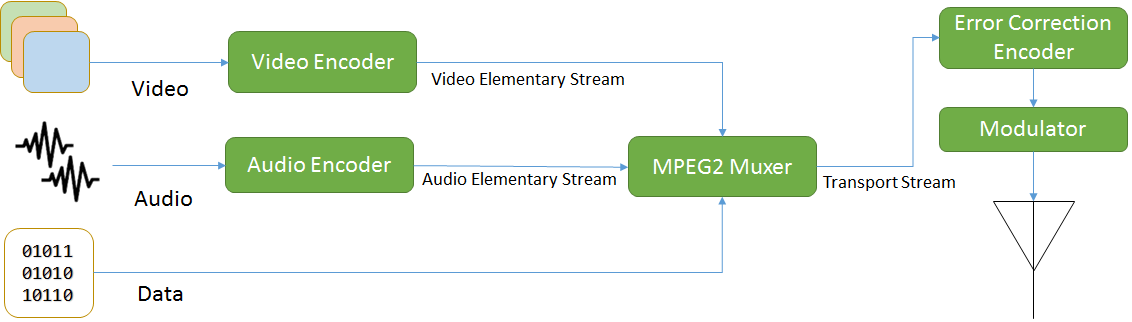
\includegraphics[width=1\linewidth]{pictures/diagrama_blocos_tvd.png}
\label{fig:diagrama_blocos_tvd}
\end{figure}
 
De l'autre côté du canal, le récepteur est conçu de manière à ce que, après passage de la couche de correction d'erreur, un \textit{démultiplexeur} prend le flux composé et le sépare de nouveau dans les flux binaires élémentaires. Ils sont ensuite envoyés aux décodeurs et aux dispositifs de sortie audiovisuels.

Il serait certainement troublant pour le spectateur de regarder les contenus vidéo ou audio en différé, sans synchronisation. Ainsi, un défi de ce schéma de multiplexage est de synchroniser la reproduction de tous les flux de média. Pour ce faire, des labels d'horodatage de présentation sont ajoutés périodiquement dans les flux afin qu'ils puissent être reproduits au même temps.

\section{Objectif et méthodologie}

L'objectif de ce projet est de développer un outil simple, mais flexible, pour gérer la couche des systèmes de la norme SBTVD. Fondamentalement, en utilisant cet outil on est capable de produire un fichier binaire compatible avec le système SBTVD, contenant un flux de transport qui peut être utilisé pour diffuser du contenu audiovisuel  dans des récepteurs appropriés. Beaucoup de solutions commerciales pour cet objectif sont disponibles sur le marché, de sorte que la cible ici n'était pas de développer un produit de consommation, mais plutôt quelque chose de plus académique, éducatif, où la plupart des configurations peuvent être modifiées selon les besoins de l'utilisateur.

Le client interne principal à l'université (UFRGS) est l'équipe du projet \textit{set-top-box} SBTVD, qui développe un boîtier décodeur du système SBTVD dans une architecture \textit{System on Chip} sur FPGA. Pour exécuter les tests de l'ensemble du système, les flux de transport avec différentes configurations de multiplexage doivent être diffusées à fin de tester le décodeur sur tous les cas prévus dans la norme.

Le LaPSI (Laboratoire de Traitement du Signal et Images) fait partie du Département d'Ingénierie Électrique (DELET) de l'Université Fédérale du Rio Grande do Sul (UFRGS) et du Programme d'Études Supérieures en Ingénierie Électrique (PPGEE). L'équipe de travail est actuellement composé de cinq enseignants, deux doctorants, 3 masters of science, 3 stagiaires et quatre employés, ainsi que la présence d'étudiants exerçant des activités de stages et projets de fin d'études.

Le laboratoire a été créé en 1991 avec l'objectif de combler l'Université dans la recherche au traitement du signal et images. En raison de l'importance atteinte par ces domaines de recherche de nos jours et aux progrès de l'électronique et des télécommunications, le laboratoire fonctionne maintenant aussi dans plusieurs autres domaines de recherche, tels que les tests de systèmes "system-on-chip" (SoC) et projets de la microélectronique analogique et numérique.

Le flux de travail du projet a été séparé en trois étapes, selon le descriptif suivant. La première étape a consisté d'une recherche bibliographique à fin d'étudier la norme ABNT NBR15603, ainsi que les références y comprises à la norme ISO/IEC 13818-1 et à la norme ARIB STD-B10. Dans cette étape, l'objectif était de comprendre comment la couche système devrait fonctionner et identifier les composants du multiplexeur qui étaient obligatoires et facultatifs. Une fois que les composants obligatoires étaient connus, les contraintes ont pu être définies. Cependant, si des structures obligatoires sont qu'à titre d'information et son absence ne bloque pas le fonctionnement du système, elles peuvent être laissés au développement futur.

La deuxième étape a envisagé définir le point de départ du développement de l'outil. Aux premières semaines de cette étape, quelques heures de travail on été consacrées à une recherche sur des outils existants aux repositoires d'applications \textit{open-sources} en ligne. Cela a été fait parallèlement à une évaluation de la possibilité de développer l'outil à partir de zéro, parce que d'autres chercheurs dans le laboratoire avaient déjà fait des recherches et avaient conclu que les outils libres trouvées, même avec des modifications, ne pourraient pas gérer les flux selon le standard SBTVD. Au cours de recherches menées par l'auteur lui même, des outils modifiables et avec des fonctionnalités réutilisables ont été identifiés. Ainsi, au lieu de développer l'outil à partir de zéro, il a été décidé de profiter d'un \textit{framework} existant.

Finalement, étant décidé qu'un outil existant serait modifié, la troisième étape a consisté du développement des fonctionnalités manquantes de l'outil choisie de l'étape deux, tout en respectant les contraintes définies à l'étape un, afin de la rendre compatible avec le SBTVD. Pour valider le projet, les fonctionnalités ont été testés sur différents récepteurs.

L'objectif technique du projet est de fournir un outil qui crée des flux de transport avec trois caractéristiques principales: présentation audiovisuelle synchrone, conformité à la norme SBTVD et possibilité d'envoi de multiples services. Les chapitres que suivent décrivent chacune des étapes citées ci-dessus, en détaillant les démarches suivies et les résultats obtenus.

\section{Norme ISO/IEC 13818-1}
\label{iso13818}

L'objectif principal de la norme ISO/IEC 13818-1 est de décrire la conversion des multiples flux de bits élémentaires (\textit{Elementary Stream}, en anglais, ou ES) en un seul flux de transport (\textit{Transport Stream}, en anglais, ou TS) enveloppant des données vidéo et audio, ainsi que des informations supplémentaires responsables de déballer les flux de données. De même que d'autres normes ISO/IEC, le texte ne précise que le côté décodage/démultiplexage de la chaîne de transmission, laissant les architectures des étapes de codage/multiplexage à la décision du fabricant.

Certains concepts doivent maintenant être décrits brièvement au lecteur. Le premier est le programme (\textit{program}, en anglais), ou service (homonyme, en anglais), qui est formé par un ensemble d'éléments de programme, qui à leur tour sont appelés les flux élémentaires. Ils peuvent partager une base de temps et donc seront reproduits simultanément. Ceci est équivalent à la notion de chaîne de télévision analogique, dans laquelle un diffuseur envoie un flux vidéo et un ou deux flux audio pour le spectateur. Le second est le \textit{PID}, qui est une étiquette attribuée par la couche système à chaque charge différente (\textit{payload}, en anglais) transportée dans le TS, quelque soit son origine ou type. Chaque table d'information a son propre PID, chaque flux élémentaire également. Le concept ici est similaire à un pointeur, dans la programmation: lors de la réception d'un paquet TS, le démultiplexeur lit le PID du paquet et pousse sa charge utile au tampon(\textit{buffer}, en anglais) approprié afin que les informations soient enchaînés avec des paquets précédemment reçus avec la même PID.

La norme définit deux architectures qui doivent être appliqués dans différentes situations. La première consiste à être utilisé dans des situations sans erreur, comme le stockage dans disques numériques, et ne seront plus discutés. L'autre architecture, adaptée aux canaux de transmission susceptibles à erreurs, est appelé le flux de transport. Le paquet du flux de transport a une longueur fixe et est considérablement petit en longueur (188 octets), ce qui le rend facile d'être protégé par les codes correcteurs d'erreur, afin d'assurer la transmission à travers les canaux défectueux. Des informations plus détaillées peuvent être obtenues dans le rapport complet du projet, en anglais, également disponible.

\subsection{Entête du Transport Stream}
\label{ts_header}

La structure principale du Transport Stream MPEG2 est un paquet de taille constante. Le flux est constitué de paquets concaténés. La \autoref{fig:TS_iso13818} montre les éléments qui sont présents dans un paquet, la valeur sous chaque champ est sa longueur en bits. Dans le tableau, on peut voir que le paquet est formé par 188 octets de données. L'en-tête obligatoire dispose de 4 octets, commence au champs \textit{sync byte} et va jusqu'au \textit{continuity counter}. La charge utile du paquet peut également contenir le \textit{adaptation field}, une sorte d'extension de l'en-tête, avec des données supplémentaires qui aident à décoder et à présenter les flux en synchronisation. Outre les 4 octets obligatoires de l'en-tête, les 184 autres octets peuvent être remplis avec une des situations suivantes: le \textit{adaptation field}, les données de PES ou les tables d'information. La présence du champs adaptation field est une option, il est couramment utilisé pour transporter des données de synchronisation et remplir l'espace vide dans le dernier paquet TS transportant un paquet PES avec des bits de bourrage. De plus amples détails sont dans le texte intégral.

\begin{figure}[!h]
\centering
\caption{Schéma de formation d'un paquet du TS.}
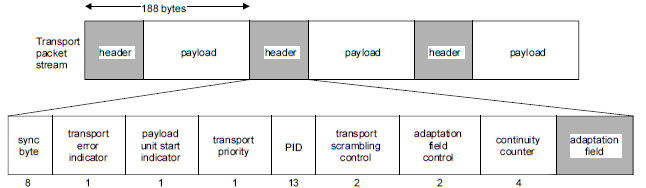
\includegraphics[width=1\linewidth]{pictures/TS_iso13818.png}
\\Source: \cite[F.0.1]{ISO}.
\label{fig:TS_iso13818}
\end{figure}


\subsection{Adaptation Field}

Le \textit{Adaptation Field} (AF) est une extension optionnelle de l'en-tête du paquet du TS. Bien qu'il soit facultatif, il contient de nombreuses informations utiles et est largement utilisé dans des applications pratiques pour transporter des informations de synchronisation et de remplir avec des octets de bourrage l'espace vide dans les paquets TS. La \autoref{fig:AdapField_iso13818} montre la concaténation des champs du \textit{Adaptation Field}. Une des caractéristiques de cette extension est que beaucoup de champs sont facultatifs, donc il y a plusieurs indicateurs qui font alterner l'existence des champs.

Le champs \textit{adaptation\hspace{0.1mm}\_\hspace{0.1mm}field\hspace{0.1mm}\_\hspace{0.1mm}length} a 8 bits et spécifie le nombre d'octets dans le \textit{Adaptation Field} immédiatement après lui-même. Quand il y a un \textit{payload} partageant le paquet TS avec le \textit{Adaptation Field}, cette valeur doit être dans la gamme 0 à 182. S'il n'y a pas de charge utile, juste le AF, la longueur doit être réglé sur 183. Pour les paquets TS transportant des données du PSE, du bourrage est généralement nécessaire dans le dernier paquet de TS utilisé parce que des paquets PES ne sont pas nécessairement des multiples de 188 octets. Le bourrage est réalisée par réglage de la longueur du \textit{Adaptation Field} de plus que la somme des longueurs des éléments de données, de sorte que les octets de charge utile restantes dans les données PES s'adaptent exactement dans l'espace gauche. L'espace supplémentaire dans le \textit{Adaptation Field} est rempli d'octets de bourrage avec la valeur \texttt{0xFF}.

Le \textit{PCR\hspace{0.1mm}\_\hspace{0.1mm}flag} informe de la présence de l'information optionnelle de synchronisation, le PCR, dans les champs \textit{program\hspace{0.1mm}\_\hspace{0.1mm}clock\hspace{0.1mm}\_\hspace{0.1mm}reference\hspace{0.1mm}\_\hspace{0.1mm}base} et \textit{program\hspace{0.1mm}\_\hspace{0.1mm}clock\hspace{0.1mm}\_\hspace{0.1mm}reference\hspace{0.1mm}\_\hspace{0.1mm}extension}. Ces champs sont enveloppés ensemble dans \autoref{fig:AdapField_iso13818} comme «PCR», avec 42 bits. Les autres champs ne seront pas décrits car ils ne sont pas cruciaux pour le fonctionnement du multiplexeur. Cependant, ils sont définis dans la norme\cite[2.4.3.5]{ISO}.

\begin{figure}
\centering
\caption{Représentation graphique du  \textit{Adaptation Field}.}
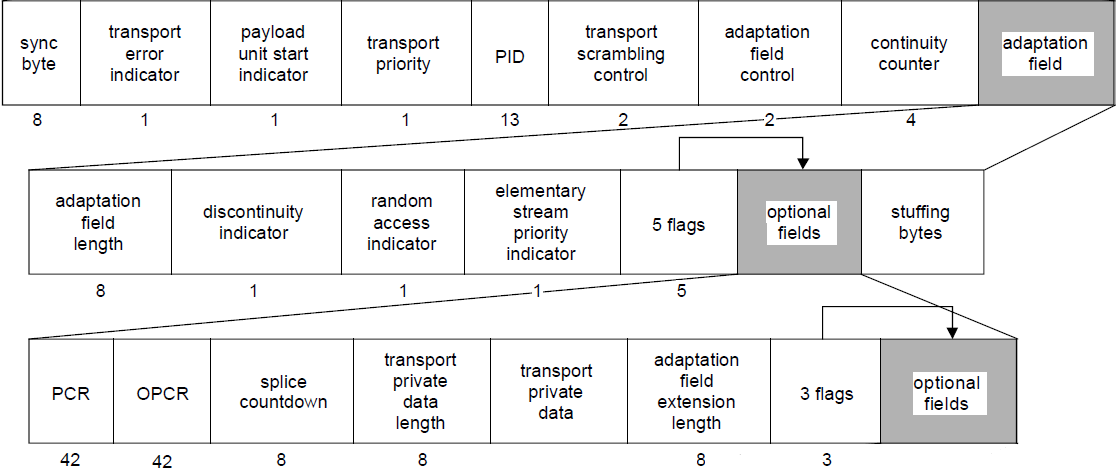
\includegraphics[width=1\linewidth]{pictures/AdapField_iso13818.png}
\\Source et droits d'auteur: \cite[F.0.1]{ISO}.
\label{fig:AdapField_iso13818}
\end{figure}

\subsection{Synchronisation}
\label{Timing}

Les données de vidéo et audio sont transportées par flux séparés qui doivent être reproduits simultanément au niveau du récepteur, de sorte que la synchronisation est crucial pour le fonctionnement d'un système de diffusion de télévision. Le modèle de temporisation introduit par la norme suppose un retard constant de bout en bout à partir de l'entrée du codeur, à travers l'émetteur, le récepteur et jusqu'à à la sortie du décodeur pour tous les flux élémentaires d'un même programme. De cette façon, il est possible d'assurer théoriquement la lecture synchrone de deux flux audio et vidéo.

Le concept clé introduit dans la norme ISO est le \textit{System Time Clock} (STC), une base de temps de référence pour tous les flux dans un même service qui est transmis. L'émetteur contrôle cette référence d'horloge pour les processus et étiquette chaque unité de présentation avec les labels d'horodatage. La valeur échantillonnée de l'horloge de référence, le PCR, est envoyée par le canal de transmission et le récepteur l'utilise pour verrouiller son propre horloge à la référence.

Si la fréquence du récepteur est la même de l'émetteur, l'encodage, le décodage et taux de présentation seront les mêmes et le système fonctionnera indéfiniment tant qu'il y ait des données à transmettre. D'autre part, si les fréquences ne sont pas verrouillés une à l'autre, une situation de débordement ou soupassement des tampons du décodeur est inévitable et finira par se produire. Si un débordement se produit, les trames seront rejetées et non présentés. Dans le cas de la vidéo encodée avec la prédiction inter-trame, si des trames rejetées seraient utilisés pour décoder d'autres trames, l'ensemble du groupe d'images serait perdu. Si un soupassement se produit, les images seraient figées ou la audio serait muette.

Il est donc important de veiller à la reconstruction de la STC dans le récepteur, car le modèle de retard constant est construit en supposant que les deux parties sont parfaitement en phase et définit les timbres de décodage et de temps de présentation selon la STC. Pour conserver le récepteur verrouillé à l'horloge de référence, une boucle à phase asservie (\textit{phase locked loop}, en anglais) est nécessaire.

\subsection{informations spécifiques au programme}
\label{iso_psi}

Les informations spécifiques au programme, ou en anglais \textit{Program Specific Information} (PSI), est un ensemble de données normatives utiles à la transmission, le démultiplexage et la présentation des flux de audio, de vidéo et de données. L'ensemble du PSI est organisée en tableaux, chacun ayant une fonction spécifique dans la norme. Les tableaux qui transportent l'information sur les PIDs qui transportent les flux vidéo et audio, appelés PAT (Program Association Table) et PMT (Program Map Table) sont obligatoires et leur syntaxe est définie par la norme ISO/IEC13818-1. La \textit{Network Information Table} est également considérée obligatoire, mais sa syntaxe n'est pas définie par la norme ISO/IEC.

Il y a une autre série de tableaux qui ne sont pas obligatoires selon la ISO13818-1, mais la ABNT NBR15603 définit comme obligatoires, comme on le verra dans la \autoref{nbr15603}. Bien que l'ISO/IEC13818-1 définit d'autres tableaux, tels que le tableau d'accès conditionnel, ils ne sont pas couramment utilisés en systèmes de radiodiffusion en clair et ont été laissés hors de la portée du projet.

Les descripteurs sont des structures utilisées pour étendre les définitions des services et de leurs éléments. La norme définit un volume considérable de descripteurs, mais ils ne sont pas tous utilisés dans des applications pratiques.

%La norme ISO définit que les tableaux PSI doivent être envoyées dans des sections et les sections peuvent être segmentés pour rentrer dans les paquets TS. Les sections ne peuvent pas avoir plus de 1024 octets, mais en pratique, le nombre d'octets pour les tables obligatoires est très en dessous de ce chiffre. Les descripteurs sont des structures utilisées pour étendre les définitions des services et de leurs éléments. Tous les descripteurs ont le même format: ils commencent par une valeur d'étiquette de 8 bits, après il y a un champ de longueur de 8 bits et finalement des octets de données de longueur variable. La norme définit un volume considérable de descripteurs, mais ils ne sont pas tous utilisés dans des applications pratiques.

\section{Norme ABNT NBR15603}
\label{nbr15603}

La norme ABNT NBR15603 est divisé en trois parties, chacune décrit une partie de la couche système du SBTVD. La plupart du contenu est une adaptation de la norme ISO/IEC13818-1, et il n'y a aucune raison de reproduire ces aspects, mais certaines particularités méritent d'être détaillées. En outre, certaines portions ont été définies sur la base de la norme japonaise ARIB STD-B10. Il existe un ensemble de tableaux obligatoires pour le SBTVD dont la syntaxe n'est pas définie dans les systèmes MPEG-2, notamment le tableau NIT, d'informations du réseau. Les PIDs qui doivent être utilisés pour transmettre les tableaux sont différents de ce qui est défini sur la norme ISO/IEC13818-1 pour quelques tableaux.

Les tableaux dont la transmission est obligatoire sont la \textit{Program Association Table} (PAT), la \textit{Program Map Table} (PMT), la \textit{Network Information Table} (NIT), la \textit{Service Description Table} (SDT), la \textit{Time Offset Table} (TOT), la \textit{Event Information Table} (EIT) et la \textit{Condition Access Table}  (CAT) (si la transmission est brouillé \footnote{Méthodes de brouillage sont utilisés pour prévenir les récepteurs sans autorisation d'ouvrir certains flux et les afficher. Ils sont généralement utilisés dans les systèmes de télévision payante, mais pas dans les systèmes de diffusion en clair.}).

Les descripteurs sont les structures de données précédemment citées, avec une syntaxe standardisée et qui augmentent la flexibilité des tableaux de porter des informations détaillées sur le système de radiodiffusion, le contenu des flux et les guides de programmation, par exemple. Les longueurs des champs de données sont flexibles, ils dépendent de l'information portée par le descripteur. S'il s'agit du descripteur du nom du diffuseur, par exemple, il doit être variable, mais si c'est plutôt un descripteur portant la fréquence centrale du canal, il doit toujours avoir la même taille. La norme ABNT définit un ensemble de descripteurs dont la présence est obligatoire dans chacun des tableaux obligatoires.

\section{Solutions disponibles et leurs limitations}

Une recherche rapide sur un moteur de recherche pour les mots clés \textit{MPEG2 TS multiplexer} renvoie une longue liste de solutions commerciales ou gratuites pour multiplexer des fichiers médias selon la norme MPEG2.

D'une part, les solutions commerciales sont généralement associées à un matériel dédié, comme la solution présentée par Imagine Communications \cite{harris}. Elles sont ciblés pour les radiodiffuseurs et sont coûteuses, de l'ordre de quelques milliers de dollars. Les principaux clients de ces solutions sont les chaînes de télévision, qui transmettent du contenu en direct, et par conséquent le codage du signal et la transmission doivent être à faible latence. Ces appareils fonctionnent en temps réel, en recevant des flux vidéo, audio et de données à travers de multiples interfaces ASI et rendent en sortie un flux multiplexé dans la norme MPEG2.

De l'autre part, les solutions libres sont des logiciels compatibles à la fois avec les plateformes PC Windows et Linux. Certains ont des interfaces graphiques pour aider son utilisation par les utilisateurs peu familiers avec les configurations en ligne de commande, certaines n'ont pas. La principale différence entre les solutions libres et les commerciales est que pour pour celles-ci, la cible n'est pas l'utilisation en temps réel, de sorte que les ordinateurs personnels sont généralement suffisantes pour exécuter les outils. Les interfaces d'entrée et de sortie sont généralement des fichiers qui stockent les flux de données binaires d'une manière séquentielle.

Afin de développer l'outil de multiplexage proposé dans le projet, des outils open-source ont été choisis pour être étudiés. Les critères de choix des solutions sont les suivants:
\begin{itemize}
\item{l'application doit être gratuit et le code source doit être sous licences open-source;}
\item{l'organisation du code source doit faciliter sa modification pour ajouter de nouvelles fonctionnalités et des données;}
\item{l'outil doit être en cours de développement, des solutions sans des mises à jour dans les 5 dernières années n'ont pas été considérés;}
\item{l'outil doit être nativement compatible avec les flux élémentaires définis dans la norme SBTVD, tels que la vidéo H.264 et la audio AAC/LATM.}
\end{itemize}

Une brève description des deux solutions qui ont atteint la plupart de ces exigences est présentée dans les paragraphes suivants. Après cela, une table synthétise leurs principales caractéristiques.

\subsection{FFMPEG}

Selon les développeurs eux-mêmes, FFmpeg est un outil polyvalent pour le codage, le décodage, la vérification et l'affichage de vidéo, audio et sous-titres. Avec un large ensemble de bibliothèques open source, permet la conversion entre différents formats, taux de trames, taille d'image vidéo, taux d'échantillonnage audio, entre autres fonctions. Il est le plus complet et soumis à des développements importants, avec des mises à jour quotidiennes organisées dans un dépôt public.

Nativement, il ne permet pas la création d'un flux TS avec de multiples services (ou programmes). Il est capable de fournir les vidéos en sortie encodées en H.264 et audio encodé en AAC-LATM, comme établit la norme ABNT. Il maintient la synchronisation entre les flux, soit en gardant les informations de synchronisation présents dans les flux d'origine ou en générant de nouvelles références temporelles. Un débit constant du flux binaire de sortie peut être réglée et le résultat est fiable.

\subsection{GPAC}

L'outil GPAC a été développé par l'école française Télécom ParisTech et a des caractéristiques similaires à FFmpeg, mais il est moins performant en garder un chronométrage précis et en maintenir un débit constant du fichier de sortie. Il prend en charge la création de plusieurs services, mais fait preuve d'un comportement aléatoire du nombre de paquets générés pour les mêmes fichiers d'entrée et les mêmes paramètres de configuration. Par exemple, pour les mêmes fichiers d'entrée avec 10 secondes de durée et les mêmes paramètres d'entrée, l'outil a été testé dix fois et a généré de 7 à 15 secondes de flux binaire de sortie, ce qui suggère une manque de contrôle de débit.

\begin{table}[!htpd]
\caption{Comparaison des Solutions Disponibles}
\begin{center}
\begin{tabular}{|c|c|c|c|}
\hline
Outil & Services Multiples & LATM & Synchronisation\\
\hline
FFmpeg & NON & OUI & OUI\\
\hline
GPAC & OUI & NON & NON\\
\hline
\end{tabular}
\label{tab_comparison_tools}
\\Source: Tests faits par l'auteur.
\end{center}
\end{table}

\subsection{Choix de la Solution}

Même si FFMPEG ne fournit pas de support natif pour les services multiples de la norme MPEG2, il a été choisi comme solution de base pour le projet, car il a été constaté que les modifications apportées au code source afin d'ajouter cette fonctionnalité étaient susceptibles d'être mises en œuvre dans le temps disponible. La fonction de synchronisation existant a favorisé le choix par cette option, aussi.

FFMPEG dispose d'une API publique qui aurait pu être utilisé pour développer une application de multiplexage à partir de zéro, mais une modification de la structure existante semblait plus rationnelle compte tenu de l'architecture orientée objet existant et le temps de développement disponible. La plupart des fonctions du multiplexeur MPEG2 existent déjà dans l'ensemble \textit{ffmpeg-formats}, mais il existent des contraintes essentielles au SBTVD qui n'y existent pas encore. Les fonctionnalités manquantes, dont le développement est l'objectif de ce projet, sont les suivantes:

\begin{itemize}
\item{support aux flux de transport MPEG2 avec services multiples;} 
\item{tableaux qui sont facultatifs dans la norme ISO/IEC, mais sont obligatoires dans le SBTVD.}
\end{itemize}

%%%%%%%
\section{Implementation du Projet}
\label{implementation}

\subsection{Le framework FFmpeg}

Le code source complet de l'application FFmpeg peut être téléchargé gratuitement à partir du site Web du projet \cite{ffmpeg}. Une fois téléchargé, ce que le développeur rencontre est un ensemble de répertoires et de fichiers. Dans le répertoire racine, il y a beaucoup de fichiers texte décrivant en détail les licences, la configuration, la compilation et l'installation de l'outil. FFMPEG est organisé dans la structure suivante: il y a quatre applications exécutables qui résultent de la compilation des paquets et leur installation: \textit{ffmpeg, ffprobe, ffplay} et \textit{ffserver}. Ces quatre applications fonctionnent sur la base de sept bibliothèques qui sont partagées entre les applications, et peuvent également être utilisés à l'extérieur de FFMPEG via l'API publique.

Les bibliothèques gèrent les fonctionnalités de l'outil, qui sont essentiellement l'encodage, le décodage, le filtrage, le multiplexage et le démultiplexage des flux médias. La bibliothèque \textit{libavformat} est responsable des fonctions de multiplexage, et son multiplexeur est compatible avec les contraintes de la ISO/IEC 13818-1. Même si une application peut être développée en utilisant les fonctions de l'API publique, le développement de FFmpeg est fait suivant les concepts de la programmation orientée objet, de manière que les interactions entre les modules sont faciles à comprendre, même pour un lecteur débutant sur le code. Ce qui suit est une description basique de l'outil. Tout le code est en langage C, sauf indication contraire. Des références pour les notations du langage C utilisés ici sont largement disponibles sur Internet \cite{cpp_reference} ou sur les livres \cite{ritchie}.

\subsubsection{Variables et Structures}

%The structures used by the multiplexer that represent the definitions on the standard are \texttt{MpegTSSection} for the tables, \texttt{MpegTSService} for the services, \texttt{MpegTSWrite} for the Transport Stream itself and \texttt{MpegTSWriteStream} for the streams.

%\texttt{MpegTSSection} is the structure that represents one PSI or SI table section and holds information of the table's PID, the current continuity counter status and a pointer to the \texttt{AVFormatContext} structure. \texttt{MpegTSService} represents a service, and contains a \texttt{MpegTSSection} for its Program Map Table, a service ID, the PCR PID and a pair of control variables to manage the service's PCR transmission rate. \texttt{MpegTSWriteStream} represents one elementary stream that is sent through the TS. It has a pointer to the corresponding service, the stream PID, a continuity counter, the stream's current PTS and DTS values and the stream raw payload itself.

Les structures utilisées par le multiplexeur qui représentent les définitions de la norme sont \texttt{MpegTSSection} pour les tableaux, \texttt{MpegTSService} pour les services, \texttt{MpegTSWrite} pour le flux de transport lui-même et \texttt{MpegTSWriteStream} pour les flux élémentaires.

\texttt{MpegTSSection} est la structure qui représente une section de tableau PSI ou SI et contient des informations de PID du tableau, l'état du compteur de continuité, et un pointeur à la structure \texttt{AVFormatContext}. \texttt{MpegTSService} représente un service et contient un \texttt{MpegTSSection} pour son tableau PMT, un ID de service, le PID du PCR et une paire de variables de contrôle pour gérer le taux de transmission du PCR du service. \texttt{MpegTSWriteStream} représente un flux élémentaire qui est envoyé par le TS. Il dispose d'un pointeur vers le service correspondant, le PID du flux, un compteur de continuité, les valeurs PTS et DTS courants des flux et la charge utile (\textit{payload}) elle-même.

%The main multiplexer structure is \texttt{MpegTSWrite}, shown in \autoref{lst_MpegTSWrite}, that represents the Transport Stream itself. The structure contains the PSI tables PAT, NIT and SDT as three \texttt{MpegTSSection} structures, a dynamic array of \texttt{MpegTSServices} and many control variables, such as the counter \texttt{nb\hspace{0.1mm}\_\hspace{0.1mm}services} for the number of services contained in the TS, the desired constant multiplexing rate \texttt{mux\hspace{0.1mm}\_\hspace{0.1mm}rate} and a pair of variables to control the repeated transmission of each PSI table.

%The class diagram of those structures and their heritage relations are shown in \autoref{fig:structMpegTSSection__coll__graph}, \autoref{fig:structMpegTSService__coll__graph}, \autoref{fig:structMpegTSWriteStream__coll__graph} and \autoref{fig:structMpegTSWrite__coll__graph}.

La structure principale du multiplexeur est \texttt{MpegTSWrite}, qui représente le flux de transport lui-même. La structure contient les tableaux  PAT, NIT et SDT du PSI comme trois structures \texttt{MpegTSSection}, un tableau dynamique de \texttt{de MpegTSServices} et beaucoup de variables pour contrôler le nombre de services contenus dans le TS, le taux de multiplexage et une paire de variables pour contrôler la transmission répétée de chaque tableau du PSI.

Le diagramme de classes de ces structures et de leurs relations d'héritage sont présentés dans \autoref{fig:structMpegTSSection__coll__graph}, \autoref{fig:structMpegTSService__coll__graph}, \autoref{fig:structMpegTSWriteStream__coll__graph} et \autoref{fig:structMpegTSWrite__coll__graph}.

\subsubsection{Fonctions}

Les principales fonctions liées au processus de multiplexage sont \texttt{av\hspace{0.1mm}\hspace{0.1mm}\_\hspace{0.1mm}\hspace{0.1mm}write\hspace{0.1mm}\hspace{0.1mm}\_\hspace{0.1mm}\hspace{0.1mm}header()} pour écrire l'en-tête du TS, \texttt{av\hspace{0.1mm}\hspace{0.1mm}\_\hspace{0.1mm}\hspace{0.1mm}write\hspace{0.1mm}\hspace{0.1mm}\_\hspace{0.1mm}\hspace{0.1mm}packet()} pour écrire les paquets et \texttt{av\hspace{0.1mm}\hspace{0.1mm}\_\hspace{0.1mm}\hspace{0.1mm}write\hspace{0.1mm}\hspace{0.1mm}\_\hspace{0.1mm}\hspace{0.1mm}trailer()} pour écrire la fin du flux. La liste suivante décrit la séquence d'appels a ces fonctions:

\begin{enumerate}
	\item{Un appel à \texttt{av\hspace{0.1mm}\_\hspace{0.1mm}write\hspace{0.1mm}\_\hspace{0.1mm}header()} initialise les variables de contrôle;}
	\item{tant que des données soient disponibles dans les flux d'entrée, des appels successifs à \texttt{av\hspace{0.1mm}\_\hspace{0.1mm}write\hspace{0.1mm}\_\hspace{0.1mm}packet()} occurrent, chacun en écrivant un paquet de 188 octets dans le fichier binaire de sortie. A son tour, \texttt{av\hspace{0.1mm}\_\hspace{0.1mm}write\hspace{0.1mm}\_\hspace{0.1mm}packet()} appelle \texttt{mpegts\hspace{0.1mm}\_\hspace{0.1mm}write\hspace{0.1mm}\_\hspace{0.1mm}pes()} pour gérer le processus d'écriture du paquet courant:}
	\begin{enumerate}
		\item {\label{itm:ret_si_info} \texttt{mpegts\hspace{0.1mm}\_\hspace{0.1mm}write\hspace{0.1mm}\_\hspace{0.1mm}pes()} appele  \texttt{retransmit\hspace{0.1mm}\_\hspace{0.1mm}si\hspace{0.1mm}\_\hspace{0.1mm}info()}, qui envoie une section de tableau PSI dans un paquet du TS, s'il est temps;}
		\item {\label{itm:dts_condition} \texttt{mpegts\hspace{0.1mm}\_\hspace{0.1mm}write\hspace{0.1mm}\_\hspace{0.1mm}pes()} boucle parmi les flux et trouve celui dont la valeur courante de DTS correspond à l'intervalle courant du PCR.}
	\end{enumerate}
	\item{quand les flux d'entrée sont finis, \texttt{av\hspace{0.1mm}\_\hspace{0.1mm}write\hspace{0.1mm}\_\hspace{0.1mm}end()} libère la mémoire allouée et ferme les fichiers ouverts.}
\end{enumerate}

%Pour décider s'il est temps, dans le \autoref{itm:ret_si_info}, \texttt{retransmit\hspace{0.1mm}\_\hspace{0.1mm}si\hspace{0.1mm}\_\hspace{0.1mm}info()} utilise les variables de contrôle \texttt{*\hspace{0.1mm}\_\hspace{0.1mm}packet\hspace{0.1mm}\_\hspace{0.1mm}count} et \texttt{*\hspace{0.1mm}\_\hspace{0.1mm}packet\hspace{0.1mm}\_\hspace{0.1mm}period} de chacun des tableaux pour contrôler les taux de transmission, en incrémentant le compteur \texttt{packet\hspace{0.1mm}\_\hspace{0.1mm}count} correspondant à chaque fois que la fonction est appelée et en rendant le tableau seulement si le compteur atteint la valeur de la période\texttt{packet\hspace{0.1mm}\_\hspace{0.1mm}period};

%FFmpeg has dedicated functions to write TS packets with PSI tables. \texttt{mpegts\hspace{0.1mm}\_\hspace{0.1mm}write\hspace{0.1mm}\_\hspace{0.1mm}section()} is responsible for writing the TS packet header fields described in \autoref{ts_header}. \texttt{mpegts\hspace{0.1mm}\_\hspace{0.1mm}write\hspace{0.1mm}\_\hspace{0.1mm}section1()} is responsible for writing the common fields for all PSI tables, described in \autoref{iso_psi}.


\subsection{Nouveaux paramètres d'entrée}

%In order to provide flexibility to the user to configure the Transport Stream parameters according to his needs, several options were added to the command-line interface.

Afin d'assurer une flexibilité à l'utilisateur de configurer les paramètres de création du flux de transport en fonction de ses besoins, plusieurs options ont été ajoutées à l'interface de ligne de commande. La plupart d'entre eux matérialisent les caractéristiques physiques du réseau et leurs noms sont très liés aux définitions des normes:
\texttt{mpegts\hspace{0.1mm}\hspace{0.1mm}\_\hspace{0.1mm}\hspace{0.1mm}transport\hspace{0.1mm}\hspace{0.1mm}\_\hspace{0.1mm}\hspace{0.1mm}stream\hspace{0.1mm}\hspace{0.1mm}\_\hspace{0.1mm}\hspace{0.1mm}id}, \texttt{mpegts\hspace{0.1mm}\hspace{0.1mm}\_\hspace{0.1mm}\hspace{0.1mm}original\hspace{0.1mm}\hspace{0.1mm}\_\hspace{0.1mm}\hspace{0.1mm}network\hspace{0.1mm}\hspace{0.1mm}\_\hspace{0.1mm}\hspace{0.1mm}id}, \texttt{mpegts\hspace{0.1mm}\hspace{0.1mm}\_\hspace{0.1mm}\hspace{0.1mm}area\hspace{0.1mm}\hspace{0.1mm}\_\hspace{0.1mm}\hspace{0.1mm}code}, \texttt{mpegts\hspace{0.1mm}\hspace{0.1mm}\_\hspace{0.1mm}\hspace{0.1mm}guard\hspace{0.1mm}\hspace{0.1mm}\_\hspace{0.1mm}\hspace{0.1mm}interval}, \texttt{mpegts\hspace{0.1mm}\hspace{0.1mm}\_\hspace{0.1mm}\hspace{0.1mm}transmission\hspace{0.1mm}\hspace{0.1mm}\_\hspace{0.1mm}\hspace{0.1mm}mode}, \texttt{mpegts\hspace{0.1mm}\hspace{0.1mm}\_\hspace{0.1mm}\hspace{0.1mm}physical\hspace{0.1mm}\hspace{0.1mm}\_\hspace{0.1mm}\hspace{0.1mm}channel}, \texttt{mpegts\hspace{0.1mm}\hspace{0.1mm}\_\hspace{0.1mm}\hspace{0.1mm}virtual\hspace{0.1mm}\hspace{0.1mm}\_\hspace{0.1mm}\hspace{0.1mm}channel}.

D'autres sont utilisés comme variables de contrôle et leurs noms sont explicites: \texttt{mpegts\hspace{0.1mm}\hspace{0.1mm}\_\hspace{0.1mm}\hspace{0.1mm}final\hspace{0.1mm}\hspace{0.1mm}\_\hspace{0.1mm}\hspace{0.1mm}nb\hspace{0.1mm}\hspace{0.1mm}\_\hspace{0.1mm}\hspace{0.1mm}services} et \texttt{mpegts\hspace{0.1mm}\hspace{0.1mm}\_\hspace{0.1mm}\hspace{0.1mm}transmission\hspace{0.1mm}\hspace{0.1mm}\_\hspace{0.1mm}\hspace{0.1mm}profile}.

% ---
\subsection{Services Multiples}
% ---

\subsubsection{Introduction}

%The first proposed modification to the original FFMPEG code is to add multiple service support. The first task was to find a way to give to the multiplexer new information about how many services should be generated. This was done by creating a new command-line parameter: the option \texttt{mpegts\hspace{0.1mm}\_\hspace{0.1mm}transmission\hspace{0.1mm}\_\hspace{0.1mm}profile}.

La première proposition de modification du code original de FFMPEG est d'ajouter le support aux services multiples dans le TS crée. La première tâche était de trouver un moyen de donner au multiplexeur la nouvelle information sur le nombre de services que devrait être généré. Cela a été fait par la création d'un nouveau paramètre de ligne de commande: l'option \texttt{mpegts\hspace{0.1mm}\_\hspace{0.1mm}transmission\hspace{0.1mm}\_\hspace{0.1mm}profile}, qui crée des profils de transmission.

Deux profils ont été conçus:
\begin{itemize}
\item profil numéro «1» a été conçu avec deux services: un service Full-segment avec un flux vidéo haute définition et un flux audio, ainsi que un service 1-segment avec un flux vidéo basse définition et un autre flux audio;
\item profil numéro «2» a été conçu avec un nombre variable de services: jusqu'à cinq services, dont jusqu'à quatre avec un flux vidéo en définition standard et un flux audio; et un cinquième service 1-segment avec un flux vidéo basse définition et un autre flux audio.
\end{itemize}

Plus d'informations sur les services Full-Segment et 1-segment sont présentés dans \autoref {modulation}. Au profil 1, d'abord l'ID de service pour le service HD est calculée. Puis, un \texttt{MpegTSService} est ajouté au tableau(\textit{array}) de services dans \texttt{MpegTSWrite}. Le processus est répété pour le service 1-segment, sauf que le type de service et le numéro de programme sont codés différemment.

Profil deux n'est pas encore mis en œuvre, mais les lignes directrices sont les mêmes que pour le profil 1. Au lieu de définir la variable du nombre de services en 2, la valeur est laissée libre pour l'utilisateur de choisir et au lieu de créer seulement deux services. Une boucle parcourt la création de services jusqu'à ce qu'un compteur atteint le nombre total de services.

\subsubsection{Association des Flux aux Services}
\label{stream_mapping}

%When calling FFmpeg, the user defines the order that input streams shall be placed in the \texttt{AVFormatContext} structure with the \texttt{-map} option. This same sequence is used in the streams loops throughout the code, and defines also the order of assignment of streams PIDs. The first input stream receives the value in \texttt{mpegts\hspace{0.1mm}\_\hspace{0.1mm}pmt\hspace{0.1mm}\_\hspace{0.1mm}start\hspace{0.1mm}\_\hspace{0.1mm}pid} and the value is incremented by one for each new stream. The default value for \texttt{mpegts\hspace{0.1mm}\_\hspace{0.1mm}pmt\hspace{0.1mm}\_\hspace{0.1mm}start\hspace{0.1mm}\_\hspace{0.1mm}pid} is \texttt{0x100}.

Lors de l'appel à FFmpeg, l'utilisateur définit l'ordre dans laquele les flux d'entrée doivent être placés dans la structure \texttt{AVFormatContext} avec le paramètre \texttt{-map}. Cette même séquence est utilisé dans les boucles internes de l'outil tout au long du code, et définit également l'ordre d'attribution des PIDs aux flux. Le premier flux d'entrée reçoit la valeur donnée par un paramètre et la valeur est incrémentée d'une unité pour chaque nouveau flux.

%Streams hold the information of which service contains them with a pointer to one \texttt{MpegTSService} instance within the \texttt{MpegTSWriteStream} structure. Before the modifications of this project, since there was only one service, all the streams belonged to it. Now, the multiplexer iterates through all the streams and does a modulus operation with the stream index and the value of \texttt{mpegts\hspace{0.1mm}\_\hspace{0.1mm}final\hspace{0.1mm}\_\hspace{0.1mm}nb\hspace{0.1mm}\_\hspace{0.1mm}services} to assign alternately one stream to each service, as shown in \autoref{lst_stream_assignment}. \texttt{ts\hspace{0.1mm}\_\hspace{0.1mm}st} is the stream structure, \texttt{i} is the iteration variable.

Les structures des flux élémentaires (\texttt{MpegTSWriteStream}) portent les informations du service auquel elles appartiennent à travers d'un pointeur vers l'instance de \texttt{MpegTSService} correspondant. Avant les modifications de ce projet, comme il n'y avait qu'un seul service, tous les flux en faisaient partie. Maintenant, le multiplexeur itère parmi les flux et fait une opération modulo\footnote{Le modulo est une fonction mathématique dont le résultat est le reste de la division euclidienne de deux nombres entiers.} avec l'indice du flux et la valeur désirée de services afin d'attribuer alternativement un flux à chaque service, comme le montre \autoref{lst_stream_assignment}. \texttt{ts\hspace{0.1mm}\_\hspace{0.1mm}st} est la structure du flux et \texttt{i} est la variable d'itération.

\begin{minipage}{\linewidth}
\begin{lstlisting}[caption={Attribution des flux aux services.}, label={lst_stream_assignment}]
ts_st->service = ts->services[i % ts->final_nb_services];
\end{lstlisting}
\end{minipage}

%The mapping should be done by placing first the two video streams, then the first audio stream corresponding to the first service, then the audio stream corresponding to the second service and finally the second audio stream corresponding to the first service.

\subsection{Tableaux PSI}

Chaque fois que \texttt{retransmit\hspace{0.1mm}\_\hspace{0.1mm}si\hspace{0.1mm}\_\hspace{0.1mm}info()} est appelée, elle met à jour les compteurs pour chaque tableau et teste s'ils ont atteint la valeur de la période. Si cela est vrai, elle appelle la fonction qu'écrit le tableau dans le fichier. Pour que le multiplexeur supporte les tableaux SDT, NIT et TOT, trois séries d'appels conditionnels ont été ajoutés, similaires à celui montré dans \autoref{lst_write_table_call}.

\begin{minipage}{\linewidth}
\begin{lstlisting}[caption={Appel à \texttt{mpegts\hspace{0.1mm}\_\hspace{0.1mm}write\hspace{0.1mm}\_\hspace{0.1mm}nit()}.}, label={lst_write_table_call}]
if (++ts->nit_packet_count == ts->nit_packet_period) {
    ts->nit_packet_count = 0;
    mpegts_write_nit(s);
}
\end{lstlisting}
\end{minipage}

%To create the bitstream of the table with pointer manipulation, first an array of type \texttt{uint8\hspace{0.1mm}\_\hspace{0.1mm}t}\footnote{\texttt{uint8\hspace{0.1mm}\_\hspace{0.1mm}t} is an unsigned integer type with size of 1 byte.} with 1012 bytes is declared with name \texttt{data}. Then a pointer \texttt{q} of the same type is declared and the first address of the array is assigned to it.

%Since all the bytes in the array are stored in a contiguous memory area, it is easy to create the table bitstream by assigning the byte value of the address pointed by \texttt{q} and incrementing the pointer after each assignment, so that the next assignment is done in the next byte of the array. Since section length is dependant on how many bytes are used and length fields are at the beginning of the headers, length fields are skipped in a first pass to be filled later, and an auxiliary pointer(\texttt{len\hspace{0.1mm}\_\hspace{0.1mm}ptr}) holds the position of the length fields for the second pass. 

Pour créer les séquences de bits des tableaux, à l'aide de la manipulation des pointeurs, d'abord un \textit{array} de type \texttt{uint8\hspace{0.1mm}\_\hspace{0.1mm}t}avec 1012 octets est déclarée avec le nom \texttt{data}. Puis un pointeur \texttt{q} du même type est déclarée et la première adresse du tableau lui est affecté.

Étant donné que tous les octets dans le \textit{array} sont stockées dans une zone de mémoire contiguë, il est facile de créer le train binaire en attribuant la valeur de l'octet de l'adresse pointée par \texttt{q} et en incrémentant le pointeur après chaque affectation, de sorte que la prochaine affectation est faite dans l'octet suivant du tableau. Comme la longueur d'une section dépend de combien d'octets sont utilisés et les champs de longueur sont au début des en-têtes, les champs de longueur sont ignorés dans un premier passage et restent à remplir plus tard. Un pointeur auxiliaire (\texttt{len\hspace{0.1mm}\_\hspace{0.1mm}ptr}) garde la position du champs de longueur pour le deuxième passage.

%Section lengths are calculated in a simple way. Most of the time their value only counts the variable size part of the sections, from right after the length field and up to the end of the last byte of the section. By calculating the difference of the two pointers \texttt{q} and \texttt{len\hspace{0.1mm}\_\hspace{0.1mm}ptr}, one gets the number of bytes written including length bytes. If one subtracts the size of the length field from this difference, he easily obtains the length of the variable portion of the section.

Les longueurs des sections sont calculés d'une manière simple. La plupart du temps leur valeur ne compte que la partie variable de la taille des sections, de juste après le champ de longueur jusqu'à la fin du dernier octet de la section. En calculant la différence de valeur des deux pointeurs \texttt{q} et \texttt{len\hspace{0.1mm}\_\hspace{0.1mm}ptr}, on obtient le nombre d'octets écrits, y compris les octets de longueur. Si l'on soustrait la taille du champ de cette différence de longueur, on obtient facilement la longueur de la partie variable de la section.

% \autoref{lst_pointer_assignment} shows an excerpt of the code: the pointer assignment algorithm. \autoref{fig:pointer_assignment} shows an example of how the  algorithm works. Six of the bytes allocated to variable \texttt{data} are shown on top, empty.
% \begin{enumerate}
% \item The first \texttt{data} address is assigned to \texttt{q} , as shown by the continuous arrow.
% \item \label{itm:len_ptr1} The syntax shown assigns the value \texttt{0x10} to the address pointed by \texttt{q} and increments by one the pointed address. The continuous arrow shows the pointed address after \autoref{itm:len_ptr1} is completed.
% \item \label{itm:len_ptr2} \texttt{len\hspace{0.1mm}\_\hspace{0.1mm}ptr} stores the current position of \texttt{q}, as indicated by the dashed arrow; the address pointed to by \texttt{q} is incremented by 2 units, as indicated by the continuous arrow, to leave space to the length fields.
% \item the value \texttt{0x45} is stored in the address currently pointed by \texttt{q}, and \texttt{q} is incremented by 1 byte.
% \item after all fields are filled with data and the length of the section is known, the length is written using the auxiliary pointer \texttt{len\hspace{0.1mm}\_\hspace{0.1mm}ptr}, that remains pointing to the same position defined in \autoref{itm:len_ptr2}.
% \end{enumerate}

% \begin{figure}[!h]
% \centering
% \caption{Pointer assignment example.}
% 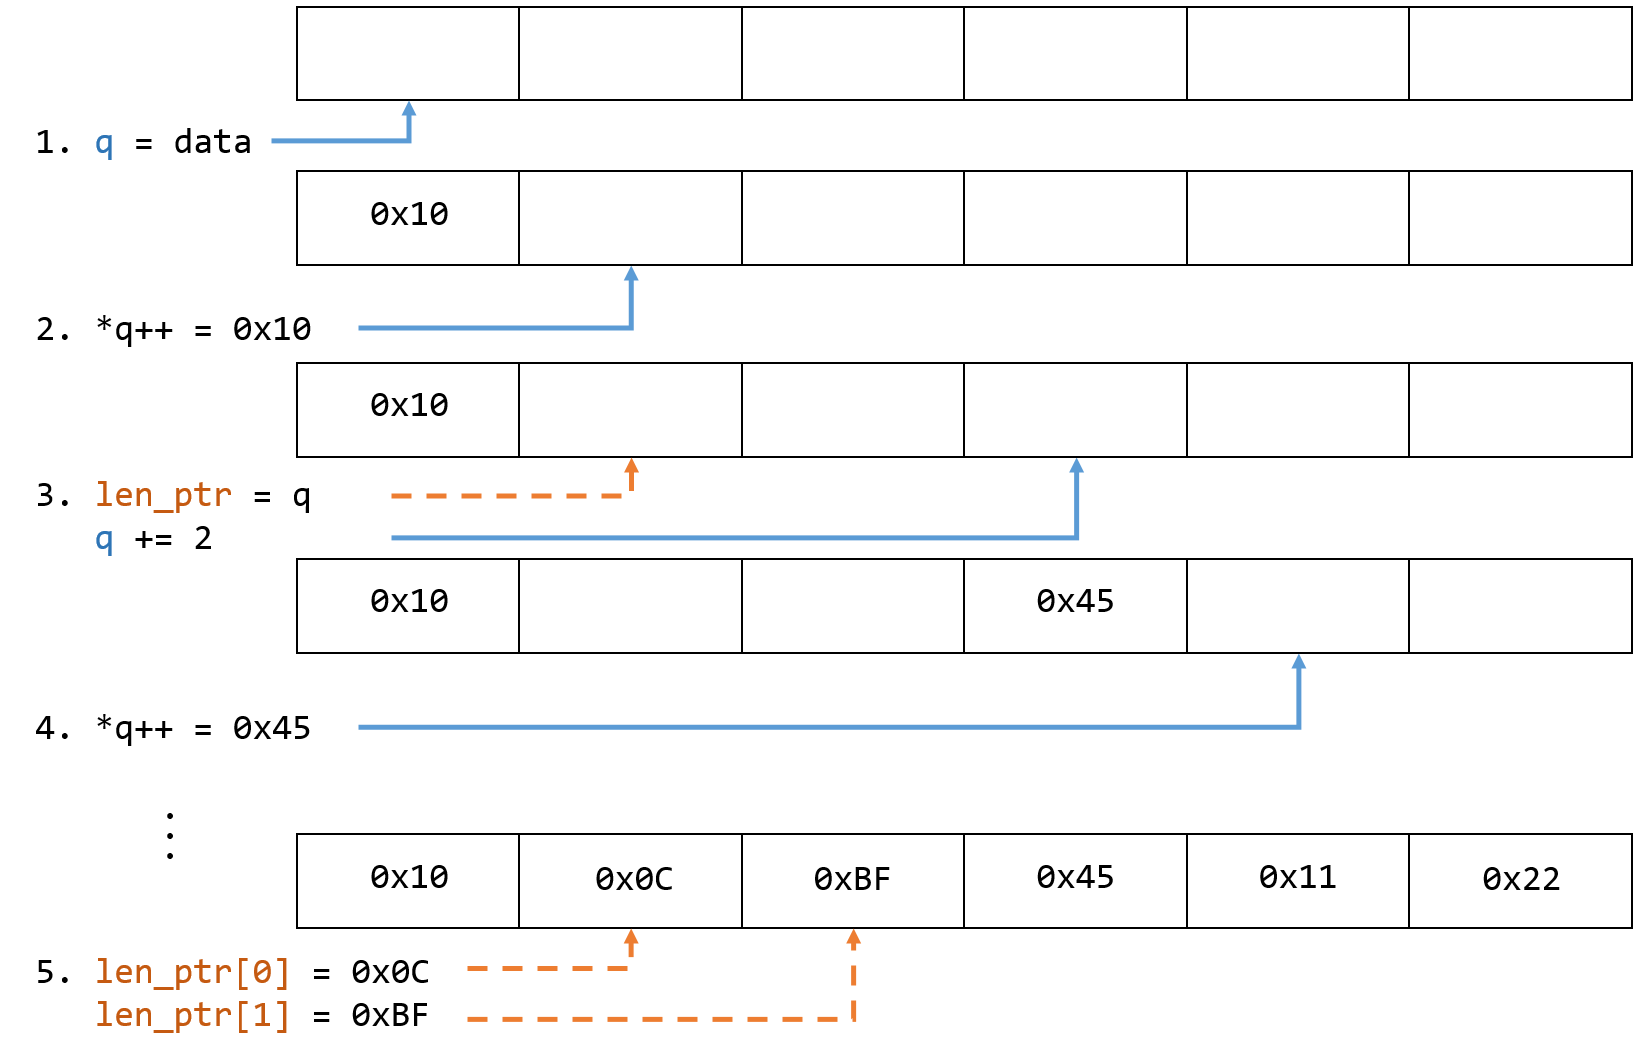
\includegraphics[width=0.8\linewidth]{pictures/pointer_assignment.png}
% \\Source: The author.
% \label{fig:pointer_assignment}
% \end{figure}

%\subsubsection{Descripteurs}

%In order to facilitate the creation of the descriptors, a prototype of C code was written. It is presented in \autoref{lst_proto_desc}. This was possible because the descriptors syntax follow a regular syntax, they always start with a tag byte, followed by a length field with one or two bytes, and followed by data bytes. The calculation of descriptors lengths use the same algorithm described in \autoref{length_calc}. All the descriptors in tables from PSI/SI which were described in theoretical sections were coded in the application.

Afin de faciliter la mise en place des descripteurs, un prototype d'un code C a été rédigé. Il est présenté dans \autoref{lst_proto_desc}. Cela est possible parce que la syntaxe des descripteurs est régulière: ils commencent toujours par un octet d'étiquette, suivi par un champ de longueur avec un ou deux octets, et suivis par des octets de données. Le calcul de la longueur des descripteurs utilise le même algorithme décrit ci-dessus. Tous les descripteurs dans les tableaux de PSI/SI cités dans les sections théoriques ont été codés dans l'application.

\begin{minipage}{\linewidth}
\begin{lstlisting}[caption={Prototype d'un descripteur.}, label={lst_proto_desc}]
	*q++ = 0x;
	_length_ptr = q;
	*q++;
	put16(&q, 0x);
	*q++ = 0x; 
_length_ptr[0] = q - _length_ptr - 1;
\end{lstlisting}
\end{minipage}

%%%%%%%
\section{Tests et Résultats}

\subsection{Environnement de Test}

Le laboratoire dispose de deux systèmes de diffusion de TV: le premier est une station EiTV Playout \cite{eitv}, qui comprend un générateur PSI/SI, un multiplexeur, un modulateur et un émetteur de faible puissance. Il s'agit d'une solution commerciale, qui satisfait aux exigences techniques de la SBTVD mais dont le code source n'est pas ouvert à la contribution. Comme entrées, on fournit un ou plusieurs flux TS, chacun avec un seul service, sous forme de fichiers binaires. Il ne permet pas que les fichiers TS d'entrée contiennent multiples services.

Cette limitation a été une motivation au développement du projet. Cette solution n'est pas complémentaire au projet, car elle ne permet pas l'envoi de multiples services dans le même TS. Il est utile, d'autre part, pour vérifier la synchronisation des flux audio et vidéo.

L'autre solution disponible est la carte PCI Dektec DTA-115, avec un modulateur numérique, qui est installé dans un poste de travail PC avec Ubuntu Linux. Ce dispositif est beaucoup plus adapté aux objectifs du projet, parce qu'il reçoit un fichier binaire avec un Transport Stream multi-services et effectue les étapes de modulation et transmission. La sortie du modulateur est évidemment en radio-fréquence, un connecteur RF qui est actuellement connecté à une antenne UHF. Une description complète de la carte est disponible dans le site Web du fabricant \cite{dektec}. Le contrôle de la carte se fait en utilisant le logiciel StreamXpress, fourni par son fabricant.

Deux dispositifs de visualisation sont disponibles pour chaque type de service: un téléviseur LCD Philips et un \textit{set-top-box} EiTV pour la réception full-segment, et pour la réception 1-segment un téléviseur numérique portable Lenoxx et un téléphone portable Samsung avec télévision numérique. En outre, un récepteur PixelView USB PenTV reçoit les transmissions Full-segment et 1-segment attaché à un poste de travail Linux. Avec le récepteur USB, les flux de transport complets sont capturés puis analysés à l'aide de deux logiciels gratuits: \textit{MPEG-2 TS Packet Analyser} et \textit{SBTVD Transport Stream Parser v0.32}. FFprobe est également utilisé comme un outil pour analyser les TS et afficher des informations sur les flux contenus en eux.

\subsection{Tests de Synchronisation}

Ces tests ont été faits avant toute modification dans le code source. L'objectif de ces premiers tests est de vérifier que FFmpeg, sans aucune modification, est capable de fournir un flux de transmission (TS) avec vidéo et audio en synchronisation.

Deux sources différentes de vidéo et audio ont été testées. La première source est un fichier \textit{mp4} qui contient une vidéo encodée en H.264 avec une résolution de 720x404 pixels, 23,98 trames par seconde, et le dont le son est encodé en HE-AAC avec deux canaux stéréo à un taux d'échantillonnage de 48 kHz. La deuxième source est un autre fichier \textit {mp4} avec de la vidéo H.264, taille d'image de 480x360 pixels à 29,97 images par seconde, et audio stéréo HE-AAC à 48KHz. Les deux vidéos ont été ré-encodées avec FFmpeg pour avoir en sortie une taille d'image de 1920x1080 pixels à 29,97 images par seconde, et le multiplexeur MPEG-2 a été utilisé pour créer un flux de transport avec un seul service. Le schéma fonctionnel dans \autoref{fig:test_scn_timing} montre le flux du signal.

\begin{figure}[!hb]
\centering
\caption{Flux de signal des tests de synchronisation.}
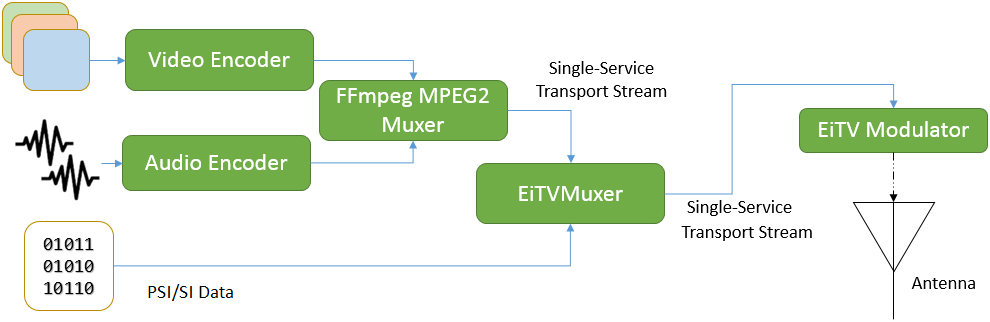
\includegraphics[width=0.9\linewidth]{pictures/test_scn_timing.png}
\\Source: L'auteur.
\label{fig:test_scn_timing}
\end{figure}

% The syntax to call ffmpeg and produce these outputs is shown in \autoref{lst_ffmpeg_single_service}. \texttt{-vcodec libx264 -r 29.97 -s hd1080 -profile:v high} set up the video codec. \texttt{-acodec aac -strict -2 -latm 1} set up the audio codec. \texttt{-t 60} tells the multiplexer to generate a TS with only 60 seconds.

% \begin{minipage}{\linewidth}
% \begin{lstlisting}[caption={Single Service TS creation with FFmpeg.}, label={lst_ffmpeg_single_service}]
% ./ffmpeg -i src.mp4 -vcodec libx264 -r 29.97 -s hd1080 -profile:v high -acodec aac -strict -2 -latm 1 -muxrate 3600000 -t 60 -mpegts_flags latm -loglevel verbose -y dst.ts
% \end{lstlisting}
% \end{minipage}

%Attention should be given to the importance of the \texttt{muxrate} parameter. In the first repetitions of this test, FFmpeg was being called without this option and the output TS ended up with a variable bitrate (VBR), which is not compliant to the MPEG2 standard and leads to a catastrophic loss of sync. When setting up the transmission parameters in EiTV control panel, the TS bitrate must be entered, so the average bitrate of the stream was applied. Since a VBR TS was being broadcast as if it had constant bitrate (CBR), whenever the output bitrate was greater than input bitrate, frames were presented faster than supposed to or skipped. On the opposite case, there were gaps without any frame and the audio would mute or the video would freeze.

Une attention particulière doit être accordée à l'importance du paramètre \texttt{muxrate}. Dans les premières répétitions de ce test, FFmpeg a été exécute sans cette option et le TS de sortie s'est retrouvé avec un débit binaire variable (VBR), ce qui n'est pas conforme à la norme MPEG2 et conduit à une perte catastrophique de synchronisation. Si un TS en VBR est diffusé comme s'il avait un débit constant (CBR), chaque fois que le débit de sortie est supérieur à celui de l'entrée, les trames vidéo ou audio sont présentées plus rapidement que le supposé ou sont ignorées. Au cas contraire, il y aurait des moments sans trames dont le son ou la vidéo se figeraient.

%After realizing the need of setting muxrate, it was necessary to know what value should be set. If an underestimated bit-rate is chosen, the PCRs and PTSs will be calculated incorrectly and frames will not be delivered at the expected frame rate. When the transmitter eventually sends the bit-stream to the air in a slower bitrate than necessary, playback will present freeze moments because there will be instants of time without video or audio to be displayed, i.e., it is as if the stream was reproduced in slow motion. On the other hand, an overestimated TS bit-rate causes the multiplexer to add too much stuffing packets into the stream and use unnecessary band.

Après se rendre compte de la nécessité de mettre \texttt{muxrate} comme paramètre, il était nécessaire de savoir quel valeur devrait être réglée. Si le débit choisi est sous-estimé, les PCR et les PTS seront calculés de manière incorrecte et les cadres ne seront pas présentés à la fréquence attendue. D'autre part, un débit binaire surestimé oblige le multiplexeur à ajouter trop de paquets de bourrage dans le flux et utiliser plus de bande que le nécessaire.

%Analyses of the local broadcast channel shown that TSs carried about 11 \% of stuffing bytes, as can be shown in the graphics in \autoref{fig:graph_rbs_dump} and \autoref{fig:graph_band_dump}. The percentages indicated in the figures refer to the amount of data in each PIDs. The PID numbers and packet counts can be seen in \autoref{tab_dumps}. In the graphs, the designation of stuffing packets is \textit{null packet}. From this information, the muxrate option was set at 3.6 Mbps, which results in an overhead of about 11 \%, as can be seen in \autoref{fig:graph_generated_dump}.

Les analyses des flux transmis par les chaînes locales montrent que environ 11 \% des octets transmis sont de bourrage, comme on peut le voir aux graphiques dans la\autoref{fig:graph_rbs_dump} et la \autoref{fig:graph_band_dump}, dans la \autoref{resultats}. Les pourcentages indiqués dans les chiffres se rapportent à la quantité de données dans chaque PID. Les numéros de PID et les chiffres de paquets peuvent être vus dans le \autoref{tab_dumps}. Dans les graphiques, la désignation des paquets de bourrage est \textit{null packet}. De cette information, l'option \texttt{muxrate} a été fixé à 3,6 Mbps, ce qui se traduit par un bourrage de l'ordre de 11 \%, comme on peut le voir dans l'analyse de la \autoref{fig:graph_generated_dump}.

% \begin{minipage}{\linewidth}
% \begin{lstlisting}[caption={Output of FFmpeg when input is as \autoref{lst_ffmpeg_single_service}.}, label={lst_ffprobe_clean}]
% Input #0, mpegts, from 'dst.ts':
  % Duration: 00:00:59.98, start: 1.445400, bitrate: 3662 kb/s
  % Program 1 
    % Metadata:
      % service_name    : Service01
      % service_provider: FFmpeg
    % Stream #0:0[0x100]: Video: h264 (High) ([27][0][0][0] / 0x001B), yuv420p, 1920x1080, 29.97 fps, 29.97 tbr, 90k tbn, 59.94 tbc
    % Stream #0:1[0x101](und): Audio: aac_latm ([17][0][0][0] / 0x0011), 48000 Hz, stereo, fltp
% \end{lstlisting}
% \end{minipage}

% FFprobe displays what is in \autoref{lst_ffprobe_clean} when analysing the output of \autoref{lst_ffmpeg_single_service}. The TS lasts 59.98 seconds and has a bitrate of 3662 kbps. It contains only one program, with program\hspace{0.1mm}\_\hspace{0.1mm}number 1, that has two streams: one video stream (PID \texttt{0x100}) and one audio stream (PID \texttt{0x101}) that comply to the requirements of the SBTVD standard.

%The streams were received in the visualization devices and the sync between video and audio was verified by watching and hearing the outputs in scenes where people were filmed while talking. Three different people stated that video and audio were in sync.

%The results were satisfactory, and although there was no employment of functionalities developed by the author, this test was necessary to ensure that the multiplexer could packetize correctly the chunks of data, as well as label the frames with timestamps in sync.

Les flux ont été reçus dans les dispositifs de visualisation et la synchronisation entre la vidéo et la audio a été vérifiée en regardant et en entendant les sorties dans les scènes où des personnes ont été filmés tout en parlant. Trois personnes différentes ont déclaré que la vidéo et la audio sont en synchronisés.

Les résultats ont été satisfaisants, et bien qu'il n'y ait pas d'emploi de fonctionnalités développées par l'auteur, ce test était nécessaire pour s'assurer que le multiplexeur de FFmpeg pourrait mettre correctement en paquets les blocs de données, ainsi que d'étiqueter les trames avec des horodateurs.

\subsection{Tests de services multiples}

%These tests were carried out after applying the implementations described in \autoref{implementation}. Their purpose is to validate the developed system. Two different sets of tests were made, one with a TS captured from a local broadcast channel with the USB receiver and the other with a TS created with the developed multiplexer.

Ces tests ont été réalisés après l'implémentation des fonctionnalités décrites dans \autoref{implementation}. Leur but est de valider le système développé. Deux séries de tests ont été réalisés, l'un avec un TS capturée à partir d'une chaîne locale avec le récepteur USB et l'autre avec un TS créé avec le multiplexeur développé.

\subsubsection{Rétransmission du TS capturé}
\label{retransmitting}

Cette première série de tests a été effectuée afin de comprendre le fonctionnement de la carte PCI Dektec et de valider son fonctionnement. Il a été fait en re-transmettant un TS qui a été capturé à partir d'un radiodiffuseur local, donc est considéré comme conforme à la norme. Le schéma simplifié de la \autoref{fig:test_scn_retrans} montre le flux du signal dans ce test.

\begin{figure}[!h]
\centering
\caption{Flux de signal des tests de retransmission de TS.}
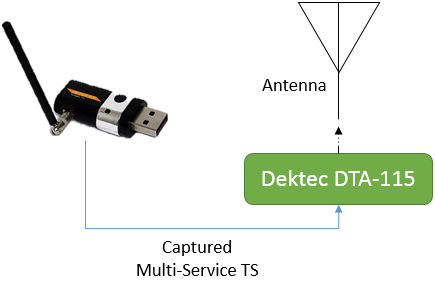
\includegraphics[width=0.5\linewidth]{pictures/test_scn_retrans.png}
\\Source: L'auteur.
\label{fig:test_scn_retrans}
\end{figure}

% The modulator board was configured with the following configuration, which is known to work as informed by previous researchers of the laboratory:

% \begin{itemize}
% \item television broadcast type, mode 3, guard interval 1/16;
% \item partial reception enabled for 1-Segment transmission on layer A;
% \item layer A configured with QPSK modulation, code rate 2/3, time interleave 2 and occupying one segment\footnote{\label{footnote_modulation}Refer to \autoref{modulation}.};
% \item layer B configured with 64QAM modulation, code rate 3/4, time interleave of 2 and occupying twelve segments\footnotemark[\value{footnote}];
% \end{itemize}

%With the captured TS file loaded in StreamXpress and these configurations set, in the program interface it is possible to select which PIDs should really be transmitted and in which layer in real-time. Several different combinations of transmitted PIDs and the status of reception in the TV and cell phone are organized in the tables presented in \autoref{resultats}. They are separated by the reception device and within each device separated by its tuning configuration. Several important information can be observed from this tables:

Dans StreamXpress, il est possible de sélectionner les PID d'un TS que seront transmis et dans quelle couche, en temps réel. Plusieurs combinaisons différentes de PID transmis et l'état de la réception de la télévision et d'un téléphone cellulaire sont organisées dans les tableaux présentés dans la \autoref{resultats}. Plusieurs informations importantes peuvent être observées à partir de ces tableaux:

% \begin{itemize}
% \item all times PAT and NIT were transmitted in layer A, so it can be noticed from \autoref{tab_manual_tuning} that the TV is capable of decoding PIDs sent in the 1-Segment layer;
% \item during blind scan, the TV can not find the broadcast channel without the NIT as proved by \autoref{tab_blind_search};
% \item in \autoref{tab_normal_operation}, without the PMT, even if the A/V ESs are sent, the TV can not open the streams;
% \item the SDT doesn't make difference to the tuning or finding PIDs, but without it the service has no name.
% \end{itemize}

\begin{itemize}
\item le PAT et la NIT ont été transmises toujours dans la couche A, de sorte qu'il peut être remarqué du \autoref{tab_manual_tuning} que le téléviseur est capable de décoder les PIDs envoyés dans la couche 1-segment;
\item pendant la recherche par chaînes, le téléviseur ne peut pas trouver le canal si la NIT n'est pas transmise, comme le prouve le \autoref{tab_blind_search};
\item dans le \autoref{tab_normal_operation}, sans le PMT, même si les ESs de audio et vidéo sont envoyés, le téléviseur ne peut pas ouvrir les flux;
\item le SDT ne fait pas de différence pour que le téléviseur trouve la chaîne ou les PIDs, mais sans elle, le service n'a pas de nom.
\end{itemize}

%With the cell phone, the results are slightly different. There is no manual tuning method, so only blind searches and normal operation tests were done. The results are:

Avec le télephone portable, les résultats sont un peu différents. Il n'y a pas de méthode de recherche manuel par chaînes, donc on ne peut utiliser que la recherche automatique. Les résultats sont:

% \begin{itemize}
% \item from \autoref{tab_cell} it can be seen that PAT presence makes no difference for the phone to open the streams. This is due to the recommendation on NBR 15608, for 1-Segment PMTs to have a default PID range;
% \item without NIT, the phone can not find the broadcast channel in blind search. If NIT is removed after blind search, the phone keeps receiving as long as PMT is still being sent.
% \end{itemize}

\begin{itemize}
\item du \autoref{tab_cell} on peut voir que la présence de le PAT ne fait aucune différence pour que le téléphone ouvre les flux. Cela est dû à la recommandation sur NBR 15608, pour que le PMT du service 1-segment soit dans une plage standardisé de PIDs, et donc il ne faut pas connaître le PAT pour trouver le PMT;
\item sans la NIT, le téléphone ne peut pas trouver la chaîne durant la recherche automatique. Si la NIT est retiré après une recherche, le téléphone ne cesse de recevoir tant que PMT soit toujours envoyé.
\end{itemize}

%This whole set of tests provides now information about what to expect when the stream generated by the developed multiplexer is broadcasted.

Tout cet ensemble de tests fournit maintenant des informations à quoi s'attendre lorsque le flux généré par le multiplexeur développé est diffusé.

\subsubsection{Transmission d'un TS ré-multiplexé avec deux services}
\label{test_remultiplexing}

L'objectif principal de cette dernière série de tests est de confirmer que le multiplexeur développé crée un TS conforme à la norme et qu'il peut être reçu et décodé correctement. Les deux entrées sont des flux de transport qui ont été capturés des chaînes locales, coupés à fin d'obtenir des ESs conformes à la norme et remultiplexés à l'aide du multiplexeur développé. L'un contient le service Full-Segment et l'autre le service 1-segment. Le flux de signal est affichée dans le diagramme en \autoref{fig:test_scn_muxing}.

\begin{figure}[!h]
\centering
\caption{Flux de signal des tests de rémultiplexation de TS.}
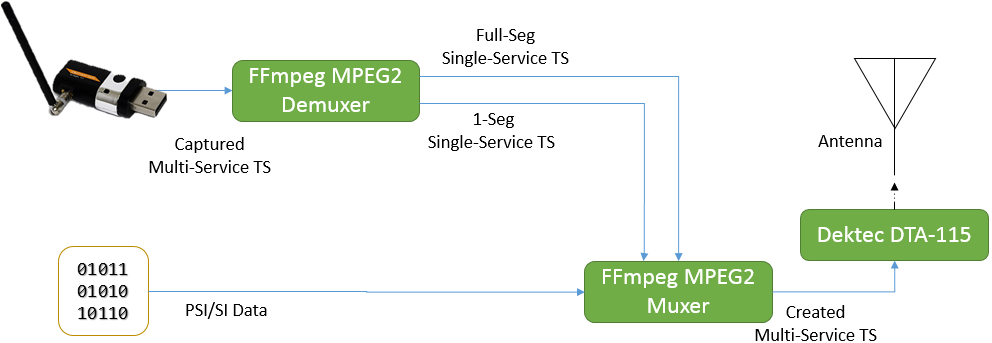
\includegraphics[width=0.8\linewidth]{pictures/test_scn_muxing.png}
\\Source: L'auteur.
\label{fig:test_scn_muxing}
\end{figure}

Le TS a été généré avec les configurations suivnates, compatibles avec le standard: original network ID 0730, area code 2970, guard interval 1/16, transmission mode 3, physical channel 20 et virtual channel 1. Le profil de transmission choisi est le «1». La \autoref{lst_ffmpeg_multi_service} montre l'appel de la commande et la \autoref{lst_ffprobe_multi_service} montre une analyse résumée de FFprobe.

\begin{minipage}{\linewidth}
\begin{lstlisting}[caption={FFmpeg command-line call to generate a multi-service TS}, label={lst_ffmpeg_multi_service}]
./ffmpeg -i /var/src/tve_HD_0406.ts -i /var/src/tve_LD_0406.ts -map 0:0 -map 1:0 -map 0:1 -map 1:1 -vcodec copy -acodec copy -mpegts_original_network_id 0730 -mpegts_area_code 2970 -mpegts_guard_interval 2 -mpegts_transmission_mode 3 -mpegts_physical_channel 20 -mpegts_virtual_channel 1 -mpegts_transmission_profile 1 -muxrate 12000000 -mpegts_flags latm -loglevel verbose -t 30 -y /home/nethome/endres/TVE_HD_LD.ts
\end{lstlisting}
\end{minipage}

\begin{minipage}{\linewidth}
\begin{lstlisting}[caption={FFprobe analysing the multi-service TS.}, label={lst_ffprobe_multi_service}]
Input #0, mpegts, from '/home/nethome/endres/TVE_HD_LD_long_1406.ts':
  Duration: 00:01:01.36, start: 1.400000, bitrate: 11972 kb/s
  Program 23360 
    Metadata:
      service_name    : SVC HD Full Seg
      service_provider: FFmpeg
    Stream #0:0[0x100]: Video: h264 (High) ([27][0][0][0] / 0x001B), yuv420p(tv, bt709), 1920x1080 [SAR 1:1 DAR 16:9], 29.97 fps, 29.97 tbr, 90k tbn, 59.94 tbc
    Stream #0:1[0x102](por): Audio: aac_latm ([17][0][0][0] / 0x0011), 48000 Hz, stereo, fltp
  Program 23385 
    Metadata:
      service_name    : SVC LD 1-Seg
      service_provider: FFmpeg
    Stream #0:2[0x101]: Video: h264 (Constrained Baseline) ([27][0][0][0] / 0x001B), yuv420p, 320x240 [SAR 1:1 DAR 4:3], 14.99 fps, 29.97 tbr, 90k tbn, 29.97 tbc
    Stream #0:3[0x103]: Audio: aac_latm ([17][0][0][0] / 0x0011), 48000 Hz, stereo, fltp
\end{lstlisting}
\end{minipage}

%The \autoref{fig:ts_parser_tve_orig_remux} shows the output of MPEG2 Parser for the original captured TS in (a), the two streams derived from it in (b) and the remultiplexed TS by this project in (c). In (a), one may notice the presence of all PSI/SI tables. In (b), only one PMT remains on each edited TS and since they were generated with the original FFmpeg, SI tables are not present(NIT, TOT), except the SDT\footnote{An SDT without all the required information is generated by FFmpeg automatically.}. In (c), the PSI/SI tables are recreated with the developed solution and the service numbers are no longer the same, since network characteristics are different from the original captured TS.

La \autoref{fig:ts_parser_tve_orig_remux} montre la sortie de MPEG2 Parser pour les TS originaux capturés en (a), les deux flux qui en dérivent en (b) et le TS remultiplexé par l'outil du projet en (c). En (a), on peut remarquer la présence de tous les tableaux PSI/SI. En (b), un seul PMT demeure sur chaque TS modifié. En (c), les tableaux PSI/SI sont recréés avec la solution développée et les numéros de service ne sont plus les mêmes, puisque les caractéristiques du réseau sont différents des TS capturés originaux.

%In \autoref{fig:ts_parser_tve_remux_pmt} the TS Parser is analysing the PMTs of the remultiplexed TS. In the left side is the PMT for Full-Segment service, where service ID \texttt{0x5B40} can be identified, the parental rating descriptor is indicating that the show if free for all ages in Brazil and the Elementary Streams described are one video of type H.264 at PID \texttt{0x100} (the primary video ES) and one AAC/LATM audio of PID \texttt{0x102}. The parser lacks the syntax of some descriptors and can not show the AAC descriptor, for example, but it can be seen that its tag is \texttt{0x7C} and content is \texttt{0x2E} as indicated by \autoref{pmt_descriptors}.

%In the right side of \autoref{fig:ts_parser_tve_remux_pmt}, the same as above is valid, but the video stream is identified as 1-segment primary video and the service number is \texttt{0x5B59}.

%It is interesting to show here that the stream mapping explained in \autoref{stream_mapping} actually worked. The first input stream was the HD video and it received the PID \texttt{0x100}. The second was the 1-Segment video, assigned PID \texttt{0x101}. The third was HD audio, that got PID \texttt{0x102}, and 1-Segment audio got PID \texttt{0x103}.

%In \autoref{fig:ts_parser_tve_remux_nit} the TS Parser is analysing the NIT of the remultiplexed TS. Since the table is too long, it was split in two parts as shown by the arrow. From the network descriptors tree, it is seen that the default network name was used in the Network Name Descriptor. The parser lacks the syntax of the System Management Descriptor. Further in the tree, one sees the value ZYA730 as the Original Network ID, the value that was passed as a parameter to FFmpeg.

Dans la \autoref{fig:ts_parser_tve_remux_pmt} TS Parser analyse les PMT des TS remultiplexés. Au côté gauche est le PMT pour le service full-segment, où le \textit{service ID} \texttt{0x5B40} peut être identifié, le descripteur de classification de contenu (équivalent à la signalétique jeunesse, en France) est indiquant que le programme  est libre à tous les âges au Brésil et les flux élémentaires décrits sont un vidéo de type H.264 au PID \texttt{0x100} (la ES de vidéo principale) et un audio AAC/LATM de PID \texttt{0x102}.

Dans la partie droite de \autoref{fig:ts_parser_tve_remux_pmt}, la différence par rapport a ce que est décrit ci-dessus est que le flux vidéo est identifié comme le flux principal du service 1-segment et le numéro de service est \texttt{0x5B59}.

Il est intéressant de montrer ici que l'adressage des flux dans le TS, expliqué dans la \autoref{stream_mapping}, a effectivement fonctionné. Le premier flux d'entrée était la vidéo HD et il a reçu le PID \texttt{0x100}. La deuxième était la vidéo 1-segment, attribué au PID \texttt{0x101}. Le troisième était la audio HD, qui a reçu le PID \texttt{0x102}, et finalement la audio 1-segment a reçu le PID \texttt{0x103}.

Dans la \autoref{fig:ts_parser_tve_remux_nit} TS Parser analyse la NIT du TS remultiplexé. Le tableau a été divisé en deux parties pour aider la visualisation, comme indiqué par la flèche. Dans l'arborescence des descripteurs du réseau, on voit que le nom de réseau par défaut a été utilisé dans le \textit{Network Name Descriptor}. L'analyseur n'a pas la syntaxe du \textit{System Management Descriptor}. En outre, dans l'arbre, on voit la valeur ZYA730 pour le \textit{Original Network ID}, la valeur qui a été passé en paramètre à FFmpeg.

%Within the TS descriptors, the TS name holds the same name of the network, as defined by the SBTVD standard. In the Transmission loop, the two services have their modulation schemes detailed, as well as the service types, numbers and IDs. In the rightmost part of \autoref{fig:ts_parser_tve_remux_nit}, the Partial Reception Descriptor points that service \texttt{0x5B59} is for 1-Segment reception. Finally, the Terrestrial System Delivery Descriptor carries many of the options passed to FFmpeg, all according to the expected.

Dans les descripteurs du TS, dans la boucle de transmission, les deux services ont leurs schémas de modulation détaillées, ainsi que les types, numéros et identifiants des services. Dans la partie droite de \autoref{fig:ts_parser_tve_remux_nit}, le \textit{Partial Reception Descriptor} indique que le service \texttt{0x5B59} est celui destiné à la réception 1-segment. Enfin, le \textit{Terrestrial System Delivery Descriptor} porte un grand nombre d'options passées à FFmpeg, le tout selon les attentes.

%In \autoref{fig:ts_parser_tve_remux_sdt} the TS Parser is analysing the SDT of the remultiplexed TS. Once again the service IDs and service types are shown, as well as the EIT scheduling flags indicating that there is neither EPG information nor EIT tables. The Service Descriptors show the service names, providers and service types.

%After this complete analysis among the PSI/SI tables generated by the code developed in the project, it can be seen that all the transmitted tables and descriptors are compliant to the standard and contain valid information. Also, the information in the tables is readable by the receptors as will be seen next. The EIT table and its descriptors, not yet implemented, did not block the system functionalities. The TOT table is currently presenting errors in operation and although it was generated, it was not broadcasted.

Dans \autoref{fig:ts_parser_tve_remux_sdt} TS Parser analyse le SDT des TS remultiplexés. Une fois de plus les identifiants de service et des types de service sont présentées, ainsi que les \textit{flags} de présence d'informations de programmation, indiquant qu'il n'y a pas d'informations EPG ni tables EIT. Les \textit{Service Descriptors} montrent les noms, les fournisseurs et les types de services.

Après cette analyse complète parmi les tableaux PSI/SI générés par le code développé dans le projet, on peut voir que tous les tableaux et leurs descripteurs transmis sont conformes à la norme et contiennent des informations valables. En outre, les informations dans les tableaux sont lisibles par les récepteurs comme on le verra ensuite. Le tableau EIT et ses descripteurs, pas encore mises en œuvre, n'ont pas bloqué le fonctionnement du système. Le tableau TOT présente actuellement des erreurs de fonctionnement et même s'il a été codé, il n'a pas été diffusé.

%The same sequence of tests of \autoref{retransmitting} was carried out for this Transport Stream. The results were similar as in the other tests, which is why the tables with results are not presented. Instead, some pictures were taken to illustrate the system working.

%\autoref{fig:video_audio_both} shows a scene with a dB meter close to the TV speaker. In the left picture are being transmitted PAT, PMTs, NIT, SDT and video ES, but no audio ES; the audio level is 61dB. In the right picture the audio ES is sent along with the other PIDs and the level increases (to 71dB), as expected.

%In \autoref{fig:info_with_without_sdt} it can be seen the effect of sending the SDT into the Transport Stream. In the left side, there is PAT, PMT, NIT but no SDT, and therefore there is no name next to the virtual channel number. In the right, on the other hand, the SDT is sent and the name "SVC HD Full Seg" is shown, which is the default name configured by the C macros in FFmpeg, as expected.

%In the left side of \autoref{fig:cell_with_sdt}, the reception on the cell phone can be seen. Overlapped to the video is the channel list with the selected virtual channel '1' and the network name describing the channel. In the right side, a manual tuning is being performed in the channel 20 of the TV and no ESs nor the SDT are being sent, only PAT, PMTs and NIT. It can be seen that the channel name is empty but there is a "good" reception level. The "Channels found" flag indicates that PAT and PMT for the HD service are present, but the blue screen points that there is no ESs to be decoded.

La même séquence de tests de réception de \autoref{retransmitting} a été effectuée pour ce deuxième flux de transport. Les résultats étaient similaires que dans les autres essais, et donc les tableaux avec des résultats ne sont pas présentés. Au lieu de cela, quelques photos ont été prises pour illustrer le fonctionnement du système.

La \autoref{fig:video_audio_both} montre une scène avec un sonomètre à proximité de l'enceinte du téléviseur. Dans l'image de gauche sont en cours de transmission PAT, PMT, NIT, SDT et ES de vidéo, sans aucun ES de audio; le niveau sonore est 61dB. Dans l'image de droite l'ES de audio est envoyé avec les autres PID et le niveau augmente (à 71 dB), comme prévu.

Dans la \autoref{fig:info_with_without_sdt}, on peut voir l'effet de l'envoi du SDT dans le flux de transport. Sur le côté gauche, sont transmis PAT, PMT, NIT, mais non le SDT, et donc il n'y a pas de nom à côté du numéro de canal. À la droite, d'autre part, le SDT est envoyé et le nom "SVC HD Full Seg" est affiché, comme prévu.

Dans la partie gauche de la \autoref{fig:cell_with_sdt}, la réception sur le téléphone portable peut être vue. On peut voir la liste des chaînes avec le canal "1" sélectionné et le nom du réseau décrivant le canal. Du côté droit, un réglage manuel est en cours d'exécution dans le canal 20 de la TV et pas de ES ni le SDT sont envoyés, seulement PAT, PMT et NIT. On peut voir que le nom de la chaîne est vide, mais un «bon» niveau de réception est disponible.

%%%%%%%
\section[Conclusions et Développement Futur]{Conclusions et Développement Futur}

La télévision est le média de communication le plus répandu au Brésil, les émissions terrestres couvrent jusqu'à 98 \% de la population et les gens comptent sur la télévision pour satisfaire leurs besoins d'information et de divertissement. En outre, les systèmes de télévision payés offrent une vidéo de haute qualité et du contenu audio haute définition, et les abonnements deviennent moins chers à chaque année. Il existe un risque important que, sans la migration des transmissions de télévision analogique terrestres vers un système numérique de haute qualité, les diffuseurs vont perdre leur audience à la télévision payé. Il est techniquement impossible de diffuser des programmes de télévision multiples ou augmenter la qualité des médias avec les systèmes analogiques existants. Il est donc nécessaire d'adopter un système de transmission numérique, à fin de fournir la solution aux problèmes techniques et commerciaux soulignés.

Après des années de discussions, le consortium formé entre gouvernement et entreprises privées a décidé de baser son système de télévision numérique, le SBTVD-T, sur celui définit par les Japonais, le ISDB-T. Les aspects techniques qui ont conduit à ce choix à la place des autres étaient la faible consommation d'énergie grâce à l'amélioration des schémas de modulation et la possibilité de diffuser vers les appareils mobiles ainsi que des dispositifs fixes dans le même canal physique.

La motivation de cette étude est née de la nécessité d'un outil pour tester la \textit{set-top box} qui est développé dans le laboratoire de traitement des signaux du département d'ingénierie électrique de l'Université. Il n'y avait pas d'outil disponible pour multiplexer et diffuser des flux élémentaires de référence, nécessaires pour tester la réception et le décodage de l'appareil développé. Par conséquent, l'objectif du projet était de développer un outil flexible et gratuit qui permet la transmission de flux multimédia selon la norme brésilienne.

Pour atteindre cet objectif, il était nécessaire d'étudier les normes ISO/IEC13818-1 et NBR15603. Après des recherches pour des solutions similaires qui existaient déjà, FFmpeg a été jugée très facilement modifiable, et a été choisi comme point de départ du développement. Comme méthodes pour valider la mise au point, un ensemble de quatre récepteurs ont été utilisés, ainsi que des outils pour analyser les fichiers de binaires générés.

Bien que le code de FFmpeg était abondamment commenté, la manque de documentation de l'outil a conduit à plusieurs erreurs aux premiers tests. Par exemple, il n'y avait aucune indication de l'unité de mesure de l'option \textit{muxrate} et il a été supposé comme «kbps» d'abord. Après des flux générés à tort, on s'est rendu compte que l'unité est plutôt «bps». En outre, le \textit{flag} LATM dans le multiplexeur n'active pas vraiment l'encapsulation du flux audio en LATM, il ne définit que la valeur d'un champs dans le descripteur de flux du tableau PMT. Le problème a été réglé en changeant le codeur audio.

En plus des tests qui ont été déjà réalisées, des expérimentations supplémentaires peuvent être faites en appliquant des images vidéo de référence à l'entrée du multiplexeur. L'état de développement actuel le permet. De plus, les étapes de codage et de multiplexage des flux qui sont faites séparément peuvent être combinés en une seule étape, de sorte que les mêmes échantillons de vidéo et audio puissent générer les deux catégories de service, full-segment et 1-segment.

En reprenant les objectifs définis au chapitre d'introduction, on peut voir que les tâches proposées ont toutes été accomplies. Le projet fournit un outil qui est conforme à la norme SBTVD, transmet la vidéo et la audio en synchronisation et permet la diffusion de multiples services. La conformité de FFmpeg à la norme SBTVD et le support des flux à services multiples sont les deux fonctionnalités ajoutées par ce projet avec succès. Les fonctionnalités de synchronisation existaient déjà, bien que personne dans le laboratoire aurait pu consacrer suffisamment d'efforts pour la faire fonctionner avant.

La conformité à la norme SBTVD a été obtenue en ajoutant les tables d'information de système qui n'étaient pas présentes dans le logiciel de FFmpeg originel. Le \textit{Network Information Table} (NIT) est crée correctement, vu que les récepteurs sont capables d'identifier l'existence du canal transmis en leur présence. Sans envoyer le tableau, cependant, la chaîne ne peut pas être identifié. Le \textit{Service Description Table} (SDT) est également correct, vu que les récepteurs parviennent à montrer les noms de service quand ils reçoivent ce tableau.

Les analyses effectuées sur les flux générés montrent la bonne formation de presque tous les descripteurs, les exceptions sont ceux dont les analyseurs n'arrivent pas à décoder. Tous les descripteurs de programmes et du système ajoutés sont interprétées correctement par TS Analyser et TS Parser, comme l'a montré les tests décrits dans les chapitres précédents.

La conformité avec le SBTVD n'est pas encore complètement mise en œuvre, cependant. Même si il a été prouvé que le flux multiplexé peut être reçu par les dispositifs et ils parviennent à le décoder correctement, le \textit{Event Information Table} (EIT), qui est obligatoire, n'est pas encore implémenté. Ce tableau n'est pas responsable du réglage du tuner, de la démodulation, ni du décodage, il est purement informative et c'est pour cela qu'il a été laissé à la poursuite du développement. Le système fonctionne sans sa présence.

Par ailleurs, le \textit{Time Offset Table} (TOT) et son descripteur obligatoire ont bien été mis en œuvre, mais quand ils ont été transmis l'information de la date et de l'heure dans les récepteurs n'a pas été mise à jour comme indiqué dans le tableau tous les temps. Pas beaucoup de temps a été consacré jusqu'à maintenant à comprendre pourquoi cet situation se passe, parce que le multiplexeur fonctionne sans cette information. Il n'existe aucune relation entre l'affichage de l'heure et la présentation des flux en synchronisation.

Surtout, les parties qui ne sont pas encore mises en œuvre sont décrites dans les chapitres théoriques et peuvent être développés avec peu d'effort, à l'aide de l'architecture FFmpeg et en profitant des algorithmes décrits par l'auteur.

Le développement futur de ce projet peut être fait pour tourner l'interface de l'outil plus convivial. Il est intéressant de créer une interface utilisateur graphique avec des listes de valeurs valides des paramètres et l'état du processus de multiplexage. En outre, une caractéristique clé encore à mettre en œuvre est le deuxième profil de transmission, qui permettra la création de flux de transport avec plus que deux services. Le profil 2 est déjà défini et décrit dans le texte, et des extraits de code peuvent être réutilisés pour mettre en œuvre cette fonctionnalité.

% ANNEXES
\appendix
\newpage
\TBannexe{Tableaux et Images des Résultats des Tests}
\label{resultats}

\begin{figure}[!h]
\centering
\caption{Distribution de paquets dans le flux transmis par le diffuseur A.}
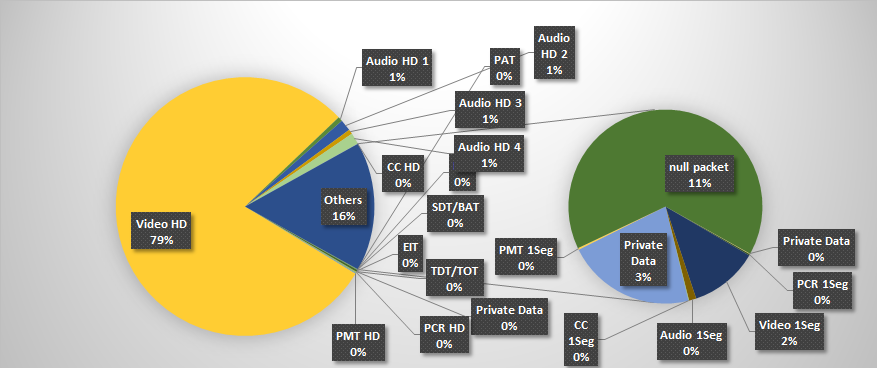
\includegraphics[width=0.9\linewidth]{pictures/graph_rbs_dump.png}
\\Source: L'auteur.
\label{fig:graph_rbs_dump}
\end{figure}

\begin{figure}[!h]
\centering
\caption{Distribution de paquets dans le flux transmis par le diffuseur B.}
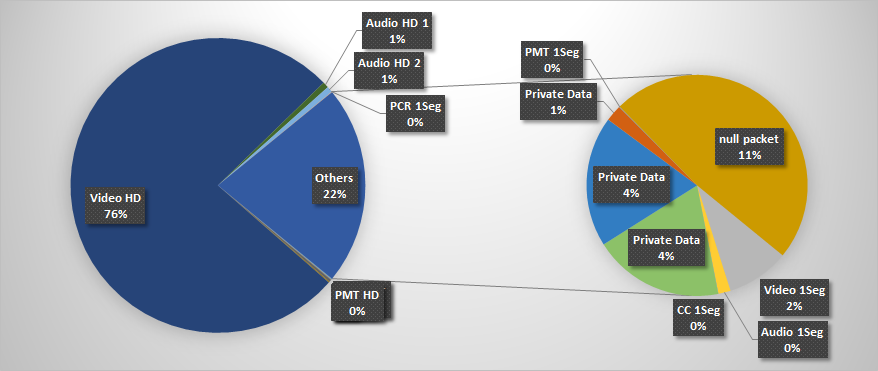
\includegraphics[width=0.9\linewidth]{pictures/graph_band_dump.png}
\\Source: L'auteur.
\label{fig:graph_band_dump}
\end{figure}

\begin{table}[b]
\centering
    \caption {Données des acquisitions de flux.}
    \begin{tabular}{|l|l|l|l|l|l|l|}
    \hline
     Diffuseur A  & Diffuseur A          & Diffuseur A    & ~ & Diffuseur B & Diffuseur B         & Diffuseur B   \\
    PID   & Type         & Compteur  & ~ & PID  & Type         & Compteur  \\ \hline
    0     & PAT          & 260    & ~ & 0    & PAT          & 100    \\ \hline
    16    & NIT          & 26     & ~ & 16   & NIT          & 10     \\ \hline
    17    & SDT/BAT      & 13     & ~ & 17   & SDT/BAT      & 5      \\ \hline
    18    & EIT          & 734    & ~ & 18   & EIT          & 10     \\ \hline
    20    & TDT/TOT      & 5      & ~ & 20   & TDT/TOT      & 2      \\ \hline
    39    & Private Data & 115    & ~ & 36   & ~            & 10     \\ \hline
    256   & PCR HD       & 452    & ~ & 39   & ~            & 10     \\ \hline
    257   & PMT HD       & 261    & ~ & 233  & CC HD        & 27     \\ \hline
    273   & Video HD     & 237551 & ~ & 256  & PCR HD       & 264    \\ \hline
    274   & Audio HD 1   & 1729   & ~ & 257  & PMT HD       & 100    \\ \hline
    275   & Audio HD 2   & 4288   & ~ & 273  & Video HD     & 76284  \\ \hline
    276   & Audio HD 3   & 1745   & ~ & 274  & Audio HD 1   & 654    \\ \hline
    277   & Audio HD 4   & 4280   & ~ & 275  & Audio HD 2   & 660    \\ \hline
    278   & CC HD        & 53     & ~ & 512  & PCR 1Seg     & 47     \\ \hline
    500   & Private Data & 51     & ~ & 529  & Video 1Seg   & 2006   \\ \hline
    512   & PCR 1Seg     & 114    & ~ & 530  & Audio 1Seg   & 394    \\ \hline
    529   & Video 1Seg   & 5551   & ~ & 549  & CC 1Seg      & 4      \\ \hline
    530   & Audio 1Seg   & 585    & ~ & 1000 & Private Data & 4169   \\ \hline
    534   & CC 1Seg      & 53     & ~ & 1001 & Private Data & 4168   \\ \hline
    900   & Private Data & 10415  & ~ & 4101 & Private Data & 521    \\ \hline
    8136  & PMT 1Seg     & 132    & ~ & 8136 & PMT 1Seg     & 26     \\ \hline
    8191  & null packet  & 31587  & ~ & 8191 & null packet  & 10529  \\ \hline
    Total & ~            & 300000 & ~ & ~    & ~            & 100000 \\ \hline
    \end{tabular}
	\label{tab_dumps}
\end{table}

\begin{figure}[!h]
\centering
\caption{Distribution de paquets dans le flux généré par le projet.}
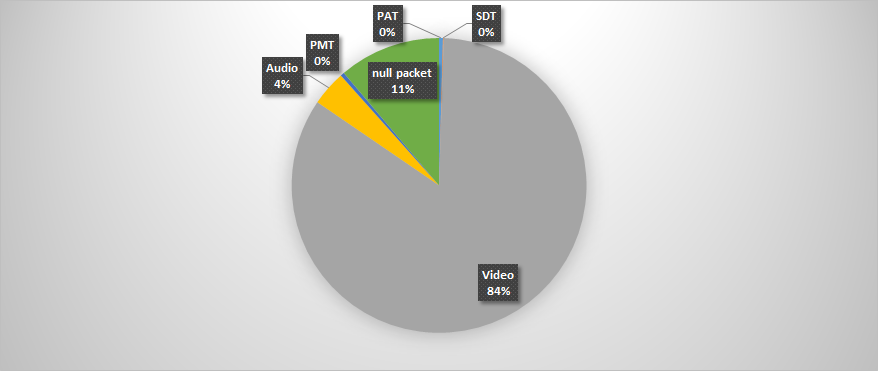
\includegraphics[width=0.9\linewidth]{pictures/graph_generated_dump.png}
\\Source: L'auteur.
\label{fig:graph_generated_dump}
\end{figure}

\begin{table}
    \caption {Téléphone portable en mode recherche par chaînes et en opération normale.}
    \begin{center}
\begin{tabular}{|l|l|l|}
    \hline
    PIDs Envoyés              & Trouve chaîne en recherche & État en opération normale \\ \hline
    NIT                    & OUI                           & "Signal too weak, retry?"  \\ \hline
    PAT, PMT, SDT, ESs d' A/V  & NON                            & Ouvre A/V                  \\ \hline
    NIT, PMT, SDT, ESs d' A/V  & OUI                           & Ouvre A/V                  \\ \hline
    NIT, PMT, ESs d' A/V       & OUI                           & Ouvre A/V                  \\ \hline
    \end{tabular}
	\label{tab_cell}
\end{center}
\end{table}

\begin{table}
    \caption {Télévision en recehrche manuel.}
    \begin{center}
\begin{tabular}{|l|l|l|l|}
    \hline
     PIDs                    & Niveau  & État de l'Écran & Nom de Service \\
	  envoyés                   & de signal & et Enceintes & Service \\ \hline
    NIT                         & 0            & Écran bleu              & AUCUN         \\ \hline
    NIT, PAT                    & Bon         & Écran bleu              & AUCUN         \\ \hline
    NIT, PAT, PMT               & Bon         & Écran bleu              & AUCUN         \\ \hline
    NIT, PAT, PMT, ESs d' A/V       & Bon         & Video et Audio en Sync  & AUCUN         \\ \hline
    NIT, PAT, PMT, ESs d' A/V , SDT & Bon         & Video et Audio en Sync  & HDTV SVC \\ \hline
    \end{tabular}
	\label{tab_manual_tuning}
\end{center}
\end{table}

\begin{table}
    \caption {Télévision en mode normal de fonctionnement.}
    \begin{center}
\begin{tabular}{|l|l|l|l|}
    \hline
    PIDs envoyés               & Ouvre Flux & "No Signal" & "No available \\
                   & d'A/V & Flag & programme" flag \\ \hline
    NIT                     & NON                & OUI              & NON                            \\ \hline
    NIT, PAT                & NON               & NON               & OUI                           \\ \hline
    NIT, PAT, PMT           & NON                & NON               & OUI                           \\ \hline
    NIT, PAT, PMT,  ES Video& OUI, video only   & NON               & NON                            \\ \hline
    NIT, PAT, ESs d' A/V   & NON         & NON               & OUI                            \\ \hline
	NIT, PAT, PMT, ESs d' A/V  & OUI, les deux         & NON              & NON                            \\ \hline
    \end{tabular}
	\label{tab_normal_operation}
\end{center}
\end{table}

\begin{table}
    \caption {Téléviseur en recherche automatique par chaînes.}
    \begin{center}
\begin{tabular}{|l|l|}
    \hline
    PIDs envoyés & Trouve chaîne \\ \hline
    NIT       & OUI           \\ \hline
    PAT, PMT  & NON            \\ \hline
    PAT       & NON            \\ \hline
    NIT, PAT  & OUI           \\ \hline
    \end{tabular}
	\label{tab_blind_search}
\end{center}
\end{table}

\begin{figure}[!h]
\centering
\caption{Sortie de TS Parser pour quatre TSs différents.}
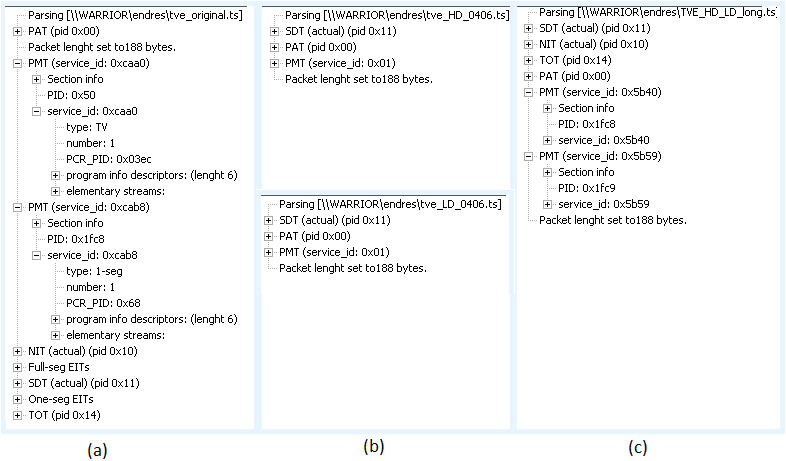
\includegraphics[width=0.9\linewidth]{pictures/ts_parser_tve_orig_remux.png}
\\Source: L'auteur.
\label{fig:ts_parser_tve_orig_remux}
\end{figure}

\begin{figure}[!h]
\centering
\caption{Analyse des PMT des flux rémultiplexés avec TS Parser.}
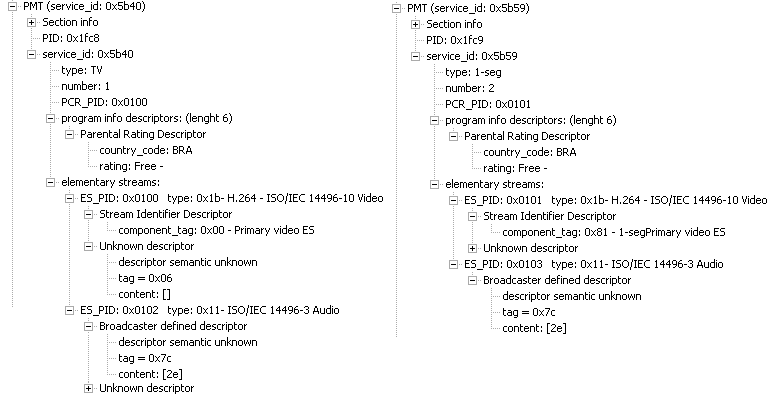
\includegraphics[width=0.9\linewidth]{pictures/ts_parser_tve_remux_pmt.png}
\\Source: L'auteur.
\label{fig:ts_parser_tve_remux_pmt}
\end{figure}

\begin{figure}[!h]
\centering
\caption{TAnalyse des NIT des flux rémultiplexés avec TS Parser.}
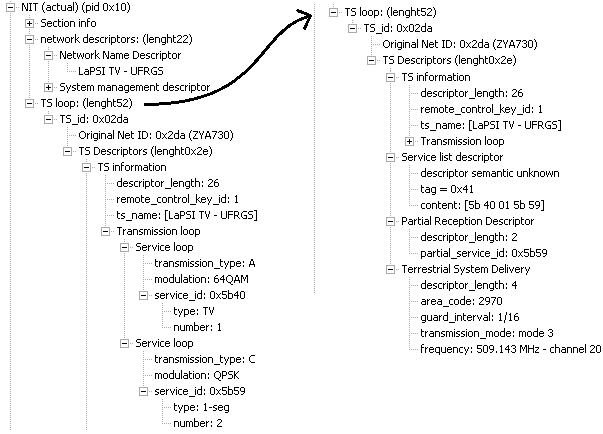
\includegraphics[width=0.9\linewidth]{pictures/ts_parser_tve_remux_nit.png}
\\Source: L'auteur.
\label{fig:ts_parser_tve_remux_nit}
\end{figure}

\begin{figure}[!h]
\centering
\caption{Analyse des SDT des flux rémultiplexés avec TS Parser.}
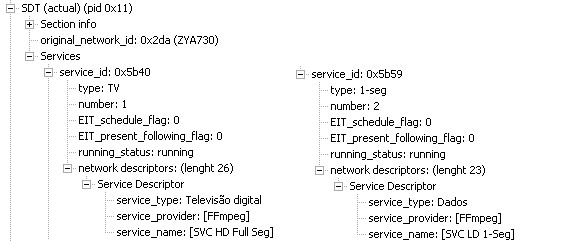
\includegraphics[width=0.9\linewidth]{pictures/ts_parser_tve_remux_sdt.png}
\\Source: L'auteur.
\label{fig:ts_parser_tve_remux_sdt}
\end{figure}

\begin{figure}[!h]
\centering
\caption{Reception de vidéo sans (gauche) et avec (droite) audio.}
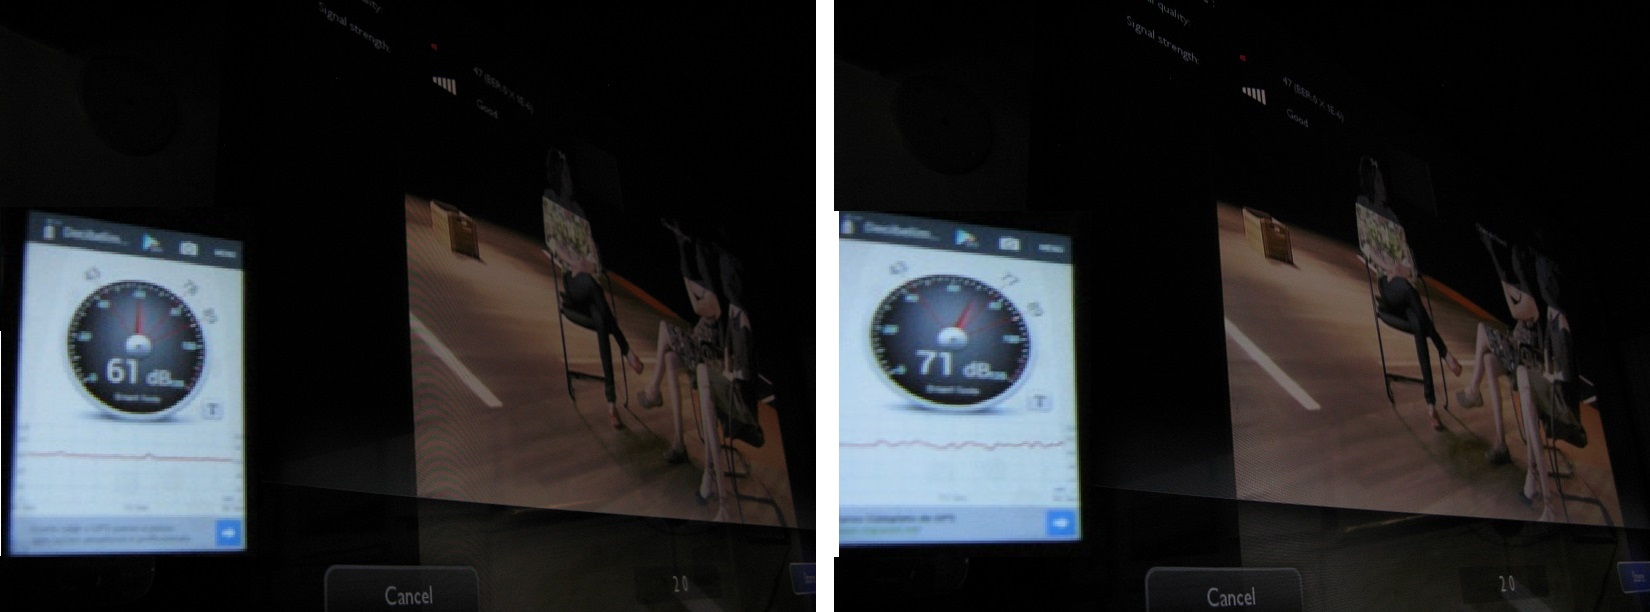
\includegraphics[width=0.9\linewidth]{pictures/video_audio_both.jpg}
\\Source: L'auteur.
\label{fig:video_audio_both}
\end{figure}

\begin{figure}[!h]
\centering
\caption{Réception sur téléphone portable (gauche) et réglage manuel du téléviseur (droite).}
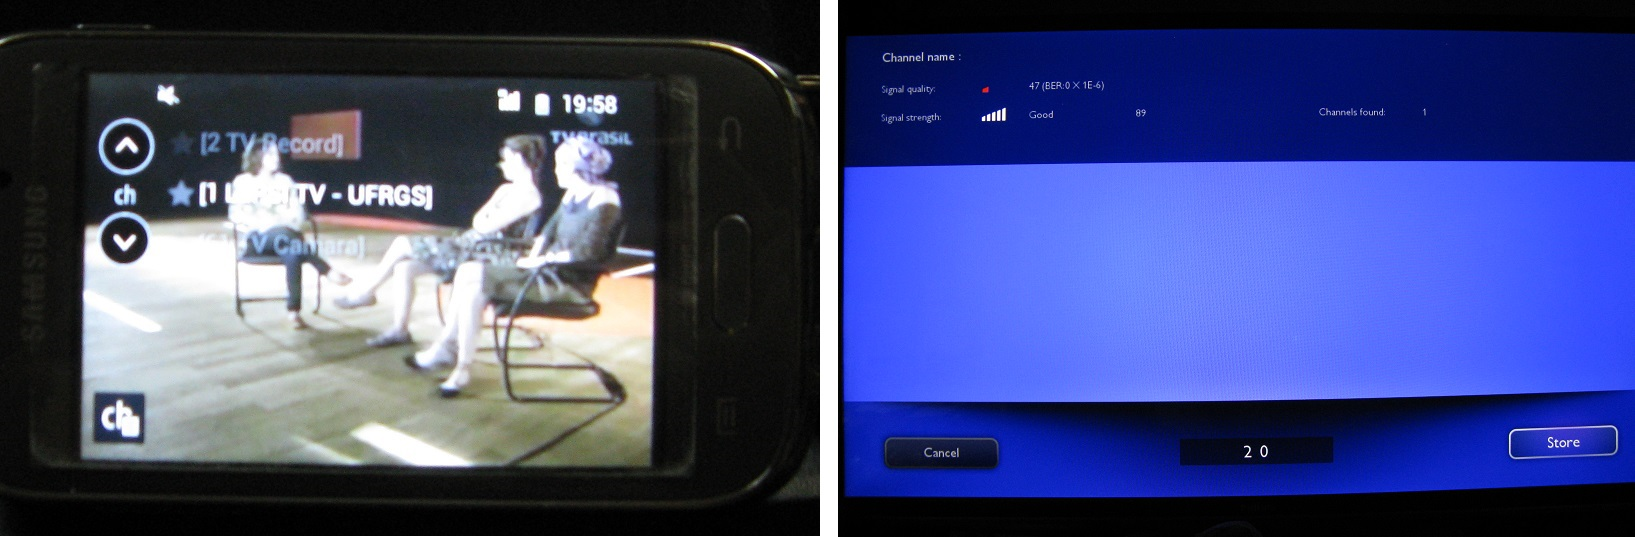
\includegraphics[width=0.9\linewidth]{pictures/cell_with_sdt.jpg}
\\Source: L'auteur.
\label{fig:cell_with_sdt}
\end{figure}

\begin{figure}[!h]
\centering
\caption{Informations du service avec (gauche) et sans (droite) le SDT.}
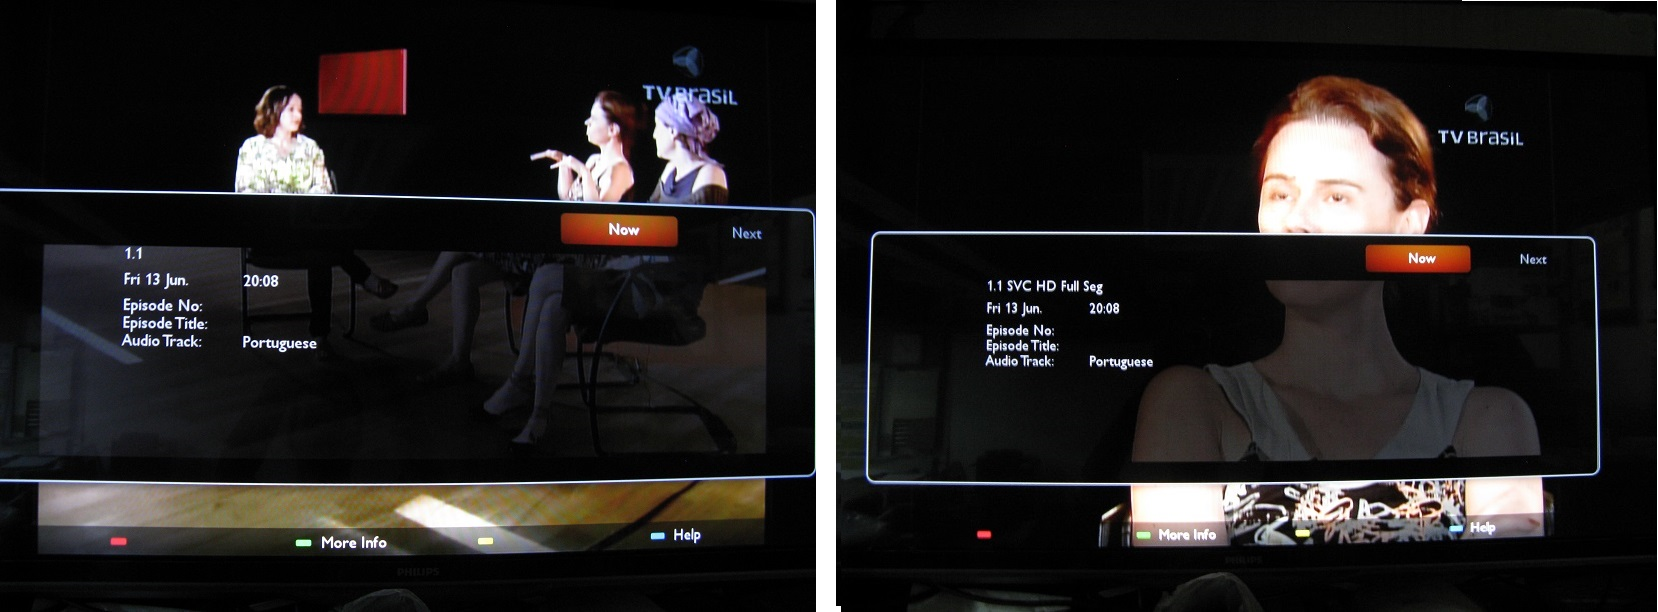
\includegraphics[width=0.9\linewidth]{pictures/info_with_without_sdt.jpg}
\\Source: L'auteur.
\label{fig:info_with_without_sdt}
\end{figure}

\newpage
\TBannexe{Diagrammes de classe de FFmpeg}
\label{diag_classe}

\begin{figure}[!b]
\centering
\caption{Diagramme de classe pour la structure MpegTSSection.}
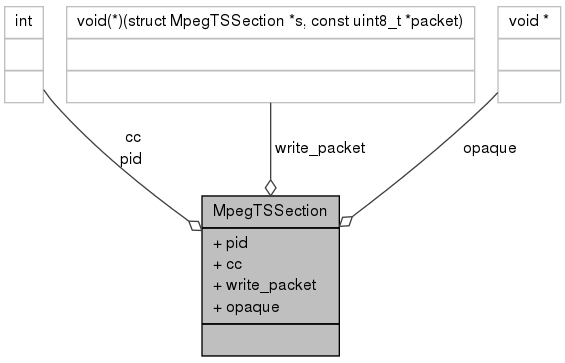
\includegraphics[width=0.8\linewidth]{pictures/structMpegTSSection__coll__graph.png}
\\Source: Généré automatiquement avec Doxygen à partir du code source.
\label{fig:structMpegTSSection__coll__graph}
\end{figure}

\begin{figure}[!b]
\centering
\caption{Diagramme de classe pour la structure MpegTSService.}
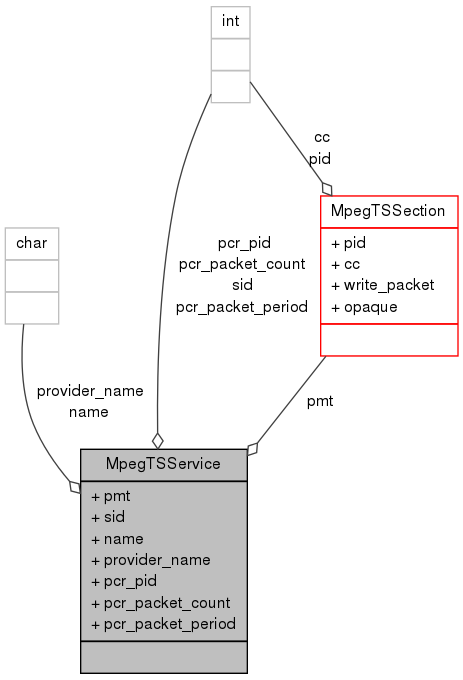
\includegraphics[width=0.8\linewidth]{pictures/structMpegTSService__coll__graph.png}
\\Source: Généré automatiquement avec Doxygen à partir du code source.
\label{fig:structMpegTSService__coll__graph}
\end{figure}

\begin{figure}[!b]
\centering
\caption{Diagramme de classe pour la structure MpegTSWriteStream.}
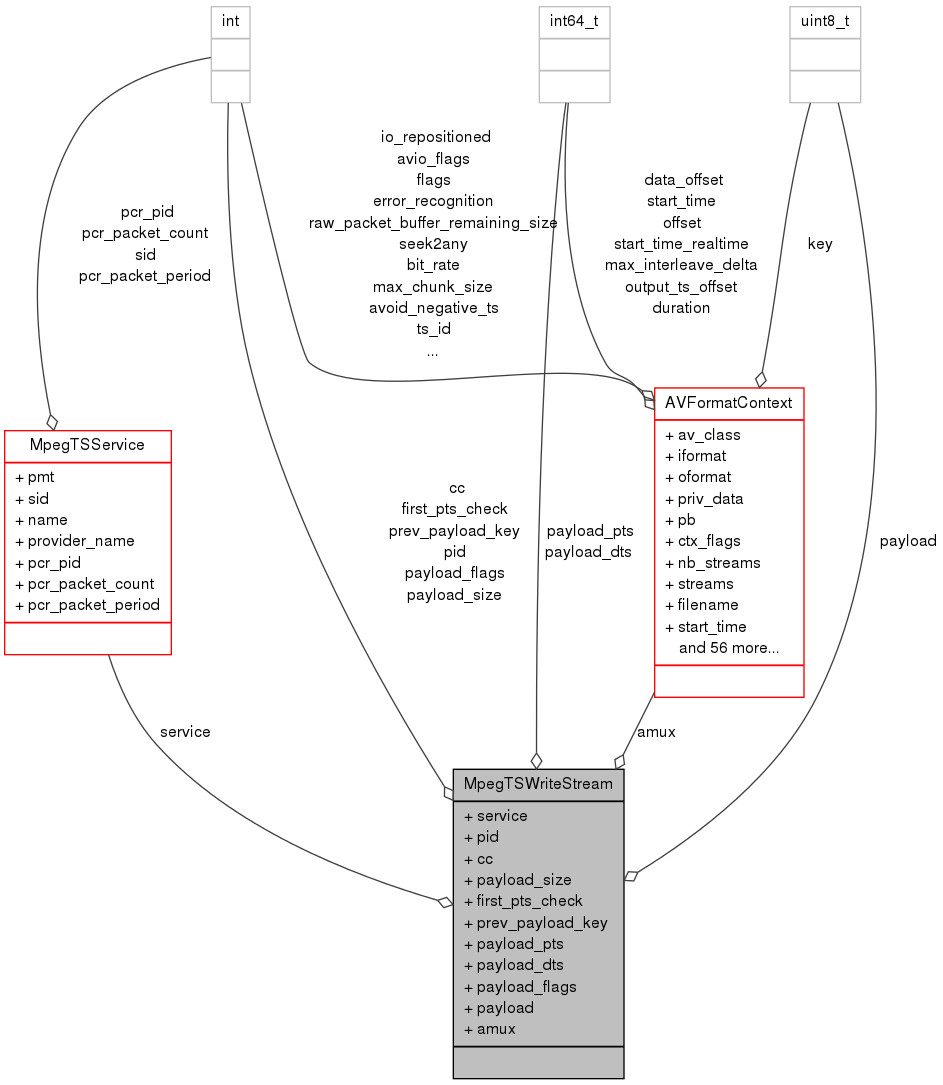
\includegraphics[width=0.9\linewidth]{pictures/structMpegTSWriteStream__coll__graph.png}
\\Source: Généré automatiquement avec Doxygen à partir du code source.
\label{fig:structMpegTSWriteStream__coll__graph}
\end{figure}

\begin{figure}[H]
\centering
\caption{Diagramme de classe pour la structure MpegTSWrite.}
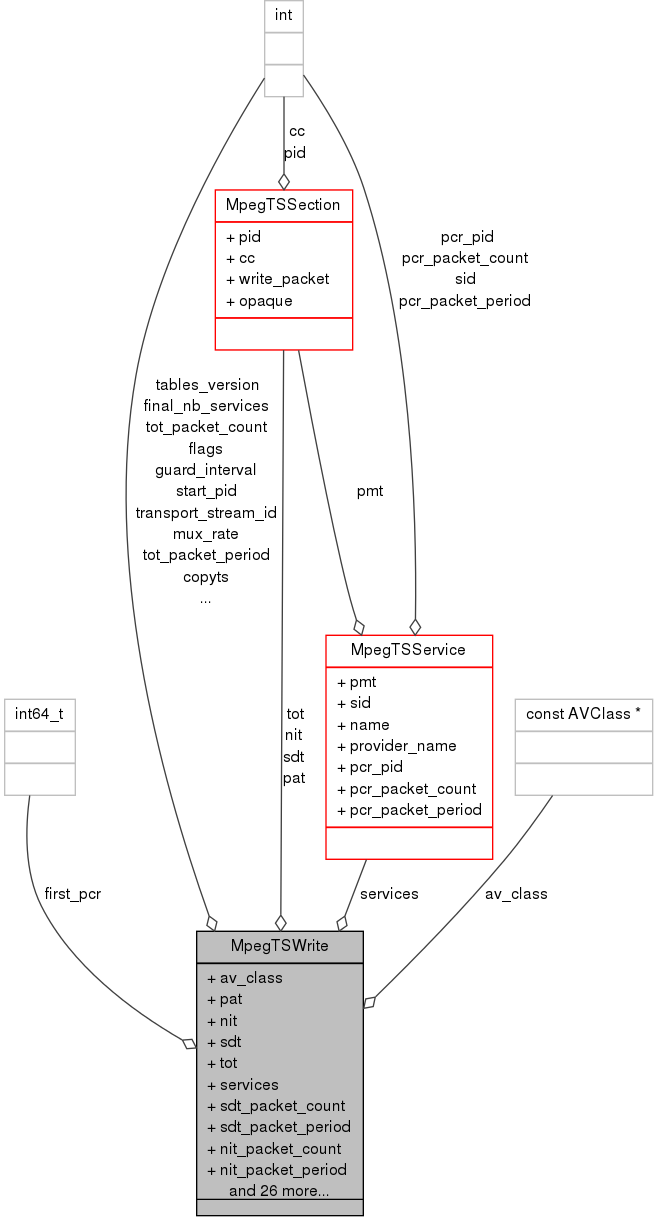
\includegraphics[width=0.7\linewidth]{pictures/structMpegTSWrite__coll__graph.png}
\\Source: Généré automatiquement avec Doxygen à partir du code source.
\label{fig:structMpegTSWrite__coll__graph}
\end{figure}

\newpage
\TBannexe{Aspects de transmission du SBTVD}
\label{modulation}

Dans le ISDB-T, un canal UHF est divisée en 13 segments de fréquence. Les récepteurs à bande étroite sont capables de décoder uniquement la fréquence(ou segment)  centrale du canal, qui sont communément appelés des récepteurs 1-segment. Les récepteurs à large bande, qui peuvent décoder tous les 13 segments de fréquence, sont appelés décodeurs full segment. \autoref{fig:ISDB-T_CH_Seg_Prog_allocation} montre la répartition des segments à l'intérieur d'un canal. «S0» est le segment central pour les tuners à bande étroite. «S1» à «S12» sont les autres segments.

Le plus la bande est étroite, le plus petite est la quantité d'informations qui peuvent être envoyées à travers elle. Les récepteurs 1-segment sont utilisés dans les appareils mobiles, et sont capables de recevoir des vidéos de basse définition (basse qualité) uniquement, avec un seul flux audio. Les récepteurs full-segment sont utilisés dans des dispositifs fixes, tels que les téléviseurs Full-HD, et sont capables de décoder la vidéo haute définition avec plusieurs flux audio.

Les schémas de modulation habituellement utilisés dans «S0» sont différents de ceux des autres segments. Comme les transmissions de TV 1-segment ciblent les appareils mobiles, la portée du signal doit être plus élevé et au plus une petite antenne dipôle est disponible au récepteur, alors une modulation QPSK est utilisée. Pour les autres segments, la quantité de données est beaucoup plus élevé, et aux clients il ne les dérange pas d'avoir une antenne amplifiée attaché à l'arrière de leur téléviseur, de sorte qu'une modulation moins robuste est appliquée, comme 64QAM.

\begin{figure}[!h]
\centering
\caption{Canal ISDB-T et ces segments.}
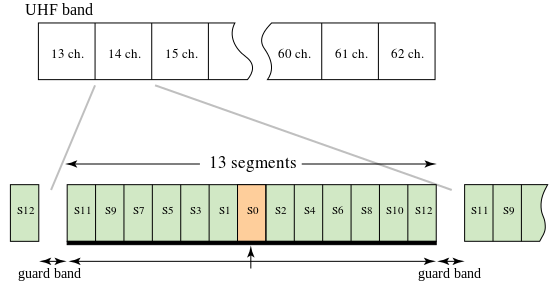
\includegraphics[width=0.8\linewidth]{pictures/ISDB-T_CH_Seg_Prog_allocation.png}
\\ Source: UnLiM, derivé de Namazu-tron, obtenu en Wikipedia \cite{ISDB_wiki}
\\ Licensed under Creative Commons 3.0 via Wikimedia Commons
\label{fig:ISDB-T_CH_Seg_Prog_allocation}
\end{figure}

%%%%%%%%%%%

%\section{Tests}
%\newpage
%\TBannexe{}
%\section{123}
%\subsection{222}
%\subsection{444}

% INDEX, RÉFÉRENCES et GLOSSAIRE
\newpage
\-\-\-
\newpage
%\TBindex
\TBbiblio{plain-fr}{includes/biblio}
%\TBglossary

\section*{Liste d'Acronymes}
\begin{itemize}
  \item[64QAM] Quadrature Amplitude Modulation avec 64 Symbols
  \item[AAC] Advanced Audio Coding
  \item[AAC-LC] Advanced Audio Coding - Low Complexity
  \item[ABNT] Associação Brasileira de Normas Técnicas
  \item[AF] Adaptation Field
  \item[ARIB] Association of Radio Industries and Businesses
  \item[CAT] Conditional Access Table
  \item[CBR] Constant Bit Rate
  \item[CRC] Cyclic Redundancy Check
  \item[DCT] Discrete Cosine Transform
  \item[DTS] Decoding Time Stamp
  \item[DTV] Digital Television
  \item[DVB] Digital Video Broadcasting
  \item[EBC] Empresa Brasileira de Comunicação
  \item[EIT] Event Information Table
  \item[EPG] Electronic Program Guide
  \item[ES] Elementary Stream
  \item[fps] frames per second
  \item[HE-AAC] High-Efficiency Advanced Audio Coding
  \item[HDTV] High Definition TV
  \item[ISDB-T] Integrated Services Digital Broadcasting - Terrestrial
  \item[IEC] International Electrotechnical Commission
  \item[ISO] International Standards Organization
  \item[ITU] International Telegraph Union
  \item[ITU-T] ITU Telecommunication Standardization Sector
  \item[LATM] Low Overhead Audio Transport Multiplex
  \item[LTE] Long Term Evolution
  \item[MPEG] Moving Picture Experts Group
  \item[NIT] Network Information Table
  \item[PAT] Program Association Table
  \item[PCI] Peripheral Component Interconnect
  \item[PCR] Program Clock Reference
  \item[PMT] Program Map Table
  \item[PTS] Presentation Time Stamp
  \item[PES] Packetized Elementary Stream
  \item[PID] Packet ID
  \item[PLL] Phase Locked Loop
  \item[PS] Parametric Stereo
  \item[PS] Program Stream
  \item[PSI] Program Specific Information
  \item[QPSK] Quadrature Phase-Shift Keying
  \item[SBR] Spectral Band Replication
  \item[SBTVD] Sistema Brasileiro de Televisão Digital
  \item[SDT] Service Description Table
  \item[SDTV] Standard Definition TV
  \item[SI] System Information
  \item[STC] System Time Clock
  \item[TOT] Time Offset Table
  \item[TS] Transport Stream
  \item[UHF] Ultra High Frequency
  \item[VBR] Variable Bit Rate
  \item[VCO] Voltage Controlled Oscillator
\end{itemize}


% ne pas modifier ! imprime la dernière page du document
\TBcoverpage
\end{document}
